\documentclass[12pt]{optlab-bachelor}
\usepackage{amsfonts}
\usepackage{amsmath,amssymb}
\usepackage{algorithm}
\usepackage{algorithmic}
\usepackage[dvipdfmx]{graphicx}

\def\年度{2017}
\def\氏名{天本 祐希}
\def\学生番号{15713004}
\def\題目{並列機械モデルにおける\\最大待ち時間最小化問題の計算論的分析}
\def\背題目{並列機械モデルにおける最大待ち時間最小化問題の計算論的分析}

\renewcommand{\bibname}{参考文献}
\newcommand{\argmin}{\mathop{\rm arg~min}\limits}

\begin{document}
\frontmatter

\chapter{はじめに}\label{c_1}
\section{研究背景}


受注生産方式では,顧客注文を受けてから,その受注製品の生産を全体の生産計画に組み込むため,どの生産拠点でいつ製造開始するかを決定する.高級自動車メーカー,SIerなど,受注生産方式を採用しており,Web サービスなどタスク処理も受注生産方式とみなすことができる.
保有する生産拠点の数と受注状況によって,受注から製造開始までの待ち時間が長くなることがあり,顧客満足度の低下や注文のキャンセルなどに繋がる.
よって,製造開始までの待ち時間を短縮させるための生産計画を立てることは重要な課題である.

また,受注生産方式では,いつ,どの製品を,いくつ製造するかなどの,顧客の注文情報をあらかじめ把握することができない.顧客の注文を受けてから,どの製品をいくつ製造する必要があるか,また,その製品がいつ注文されたのか,などの情報を把握することができる.さらに,その製品の正確な製造完了日時は,実際に製造が完了するまで把握できない.このように,注文情報があらかじめ把握できない環境をオンライン環境という.つまり,受注生産方式において,製造開始までの待ち時間を短縮させるための生産計画を立てることは,オンラインスケジューリング問題として捉えることができる.

ここで,各注文をジョブに対応させ,受注日時を処理開始可能時刻,製造期間を処理時間,受注日時と製造期間の和を納期とすると,処理開始可能時刻付き最大遅れ時間最小化問題における最大遅れ時間は最大待ち時間に対応し,JIT ジョブ荷重和最大化問題において全てのジョブを JIT で処理することは最大待ち時間が 0 の場合に対応する. 処理開始可能時刻付き最大遅れ時間最小化問題は単一機械モデルにおいて,JIT ジョブ荷重和最大化問題は無関連並列機械モデルにおいて機械数が入力の一部の場合,それぞれ強 NP 困難であることが示されている.
しかし,直接的に目的関数を待ち時間とするスケジューリング問題を扱う従来研究は,調査した限り存在しない.

% また,高級自動車メーカは,いつ,どの車種に,どのようなオプションをつけて,何台製造するか,などの顧客からの注文内容を,あらかじめ知ることはできない.注文を受けたときに初めて,その顧客がいつ,どのような車種で,どのようなオプションをつけ,何台注文したのかわかる.また,製造が完了するまで,その注文に対する正確な製造完了日を知ることもできない.
% このように,製造する製品の情報があらかじめわからない環境,処理が完了して初めて製品の情報がすべてわかる環境をオンライン環境という.
% オンライン環境において,スケジュールを決定する問題をオンラインスケジューリング問題という.対して,製品の情報すべてがあらかじめわかっている環境をオフライン環境という.
% 最大待ち時間最小化問題は,処理開始可能時刻を制約とし,最大待ち時間の最小化を目的とするスケジューリング問題である.
% 最大待ち時間を目的関数としたスケジューリング問題は,どの機械モデルにおいても未解決問題である.

\section{研究目的}
本研究では,上記の問題を最大待ち時間最小化問題として定式化した.
最大待ち時間最小化問題の拡張問題である処理開始可能時刻付き最大遅れ時間最小化問題は単一機械モデルにおいても強 NP  困難である.そのため,最大待ち時間最小化問題も NP 困難であることが予想されるが,明らかではない.
本研究では,オフライン環境における最大待ち時間最小化問題に対して以下を目的とする.
\begin{description}
  \item[目的 1 :]
  最大待ち時間最小化問題の計算複雑さを明らかにする.
\end{description}

最大待ち時間最小化問題を決定問題として定義し,機械モデルおよび機械数に着目することで,どのような特徴が問題の難しさに影響を与えるかを明らかにする.

\begin{description}
  \item[目的 2 :]
  最大待ち時間最小化問題に対する効率的解法の提案を行う.
\end{description}

各機械モデルにおける最大待ち時間最小化問題の計算複雑さに基づいて,解法の提案を行う.
また,計算機を用いて解法の実験的評価を行う.

\section{章構成}
本論文の章構成は以下である.
\begin{itemize}
  \item 第~\ref{c_2}~章では,最大待ち時間最小化問題の定式化を行なう.また,既存のスケジューリング問題との対応づけ,NP完全性の証明のために,最大待ち時間最小化問題を決定問題として定義し,定式化を行う.
  \item 第~\ref{c_3}~章では,最大待ち時間最小化問題に関連する,JITジョブ荷重和最大化問題と
  処理開始可能時刻付き最大遅れ時間最小化問題に対する従来研究の成果を,計算複雑さの観点,解法の観点から,それぞれまとめる.
  \item 第~\ref{c_4}~章から第~\ref{c_5}~章にかけて,本研究の成果を述べる.第~\ref{c_4}~章では,最大待ち時間最小化問題の計算複雑さについて述べる.
  \item 第~\ref{c_5}~章では,提案解法の紹介と,分析規模拡大のために改良した分枝限定法の紹介を行う.また,実験より得たデータから提案解法の評価を行う.
  \item 第~\ref{c_6}~章では,結論として,本研究の成果と今後の課題を述べる.
  \item 付録~\ref{c_7}では,第~\ref{c_5}~章で提案した解法の分析に用いた実験結果を載せる.
\end{itemize}

\chapter{諸定義}\label{c_2}
この章では,最大待ち時間最小化問題と待ち時間制約付きスケジューリング問題を定式化する.
また,計算複雑性クラスについて,例を挙げて紹介する.

定式化に先立ち,スケジューリング問題における機械モデルを紹介する.
各ジョブを処理する機械の性能によって,機械モデルは次のように分類され
る.まず,ジョブを処理する機械の台数について,一つの機械で処理する単一
機械モデルと,複数の機械で処理を行なう並列機械モデルに分類される.並列
機械モデルはさらに,全ての機械の性能が等しい同一並列機械モデル,機械ご
とに処理速度が異なる一様並列機械モデル,ジョブと機械の組み合わせによっ
て処理時間が異なる無関連並列機械モデルに分類される.

\section{最大待ち時間最小化問題}
最大待ち時間最小化問題とは,各ジョブの処理開始可能時刻を制約
とし,処理開始可能時刻と処理開始時刻の差の最大値の最小化を目的とするス
ケジューリング問題である.
以下では,無関連並列機械モデルについて,最大待ち時間最小化問
題を定式化する.

\begin{quote}
  \begin{description}
    \item[] {\bf 最大待ち時間最小化問題}
    \item[入力:]
    ジョブの集合 $\mathcal{J}$,無関連機械の集合 $\mathcal{M}$,
    処理開始可能時刻を返す関数 $r : \mathcal{J} \to \mathbb{N}$,処理
    時間を返す関数 $p : \mathcal{J} \times \mathcal{M} \to \mathbb{N}$
    からなる 4 項組 $(\mathcal{J}, \mathcal{M}, r, p)$.
    \item[解:] 問題の前提に基づき,スケジュールを定式化する.スケジュールは以下の条
    件を満たす $A : \mathcal{J} \to \mathcal{M}$ と $s : \mathcal{J} \to
    \mathbb{N}$ の対$(A,s)$ であり,スケジュールによって,各ジョブを,どの
    機械で,いつ処理するかを決める.
  \end{description}

  \begin{itemize}
    \item $\forall J \in \mathcal{J}\big[s(J) \ge r(J) \big]$
    \begin{itemize}
      \item 各ジョブは処理開始可能時刻以降に処理を開始する
    \end{itemize}

    \item $\forall J, J' \in \mathcal{J}\ \Big[ \big[J\ne J' \land A(J) = A(J')\big] \Rightarrow$ \\ $~~~~~~~~~~~~~~~~~~~~~~~~~~~~~[s(J), s(J)+p(J,A(J))) \cap[s(J'), s(J')+p(J', A(J'))) = \emptyset \Big]$
    \begin{itemize}
      \item 各機械は同時に複数のジョブを処理しない.
      \item 各ジョブの処理を開始すると,完了するまで中断しない.
    \end{itemize}
  \end{itemize}

  \begin{description}
    \item[目的関数:] 実行可能なスケジュール $(A,s)$ のうち,最大の待ち時間,
  \end{description}
  \begin{displaymath}
    \varphi(A,s) = \max_{J \in \mathcal{J}} \left\{s(J) -
    r(J)\right\}
  \end{displaymath}
  \begin{description}
    \item[] ~を最小とするスケジュールを求める.
  \end{description}
\end{quote}

\section{待ち時間制約付きスケジューリング問題}
待ち時間制約付きスケジューリング問題とは,各ジョブの処理開始可能時刻を制約
とし,処理開始可能時刻と処理開始時刻の差の最大値が $w$ 以下となるスケ
ジュールが存在するかを判定する問題である.
以下では,無関連並列機械モデルについて,待ち時間制約付きスケジューリング問題を定式化する.

\begin{quote}
  \begin{description}
    \item[] {\bf 待ち時間制約付きスケジューリング問題}
    \item[インスタンス : ]
    ジョブの集合 $\mathcal{J}$,無関連機械の集合 $\mathcal{M}$,
    処理開始可能時刻を返す関数 $r : \mathcal{J} \to \mathbb{N}$,処理
    時間を返す関数 $p : \mathcal{J} \times \mathcal{M} \to \mathbb{N}$,待ち時間 $w$ からなる 5 項組 $(\mathcal{J}, \mathcal{M}, r, p, w)$.

    \item[問題 : ] 実行可能なスケジュール $(A,s)$ のうち,以下の条件を満たすスケジュール $(A,s)$ が存在するかどうか.
  \end{description}

  \begin{itemize}
    \item $\max\big\{s(J) - r(J) \mid J \in \mathcal{J}\big\} \le w$
    \begin{itemize}
      \item ジョブの処理開始可能時刻からその処理を開始するまでの待ち時間は $w$ 以下.
    \end{itemize}
  \end{itemize}
\end{quote}

待ち時間制約付きスケジューリング問題を繰り返し解くことによって,最大待ち時間最小化問題も解くことができる.以下では,その手法について簡単に紹介する.

例えば,処理開始可能時刻の昇順で,任意の機械に割り当てることで,1 つ実行可能なスケジュールを作ることは可能である.
このスケジュールにおける最大待ち時間 $W_h$ は,最適解における最大待ち時間以上の値となる.
次に,$0$ と $W_h$ の中間の値 $W_h/2$ を制約付きスケジューリング問題のインスタンスとして,問題を解く.
判定が Yes のとき,最大待ち時間の値を半分 $W_h/4$ にして,制約付きスケジューリング問題のインスタンスとして,問題を解く.
判定が No のとき,$W_h/2$ と $W_h$ の中間の値 $W_h/2 + W_h/4$ を 制約付きスケジューリング問題のインスタンスとして,問題を解く.
この操作を繰り返し行うことで,最適解における最大待ち時間を有限ステップで求めることができる.
つまり,制約付きスケジューリング問題の待ち時間に対して,二分探索を有限ステップ行うことで,最大待ち時間最小化問題の最適解における最大待ち時間を求めることができる.

\subsection{既存のスケジューリング問題との対応}
以下では,最大待ち時間最小化問題もしくは待ち時間制約付きスケジューリング問題とJIT ジョブ荷重和最大化問題,処理開始可能時刻付き最大遅れ時間最小化問題との共通部分と差分をまとめる.

\begin{itemize}
  \item \textbf{JIT ジョブ荷重和最大化問題との共通部分}

  待ち時間制約付きスケジューリング問題において,待ち時間 $w$ の制約が最も強い場合,つまり,$w = 0$ のとき,各ジョブは処理開始可能時刻ちょうどで処理を開始しなければならない.このとき,待ち時間制約付きスケジューリング問題におけるすべてのジョブが JIT ジョブであるかという判定に等しい.
  JIT ジョブ荷重和最大化問題を決定問題として定義する.つまり,荷重和が $W$ 以上となるスケジュールが存在するかという問題に置き換える.このとき,$W$ の制約が最も強い場合,つまり,$W = {\displaystyle \sum_{J \in \mathcal{J}}w_J}$ のとき,すべてのジョブが JIT  ジョブであるかという判定に等しい.

  つまり,待ち時間制約付きスケジューリング問題に対して,$w = 0$ のスケジュールが存在するとき,そのインスタンスにおける JIT ジョブ荷重和最大化問題に対して,$W = {\displaystyle \sum_{J \in \mathcal{J}}w_J}$ となるスケジュールが存在する.
  また,$W = {\displaystyle \sum_{J \in \mathcal{J}}w_J}$ となるスケジュールが存在するとき,そのインスタンスにおける待ち時間制約付きスケジューリング問題に対して,$w = 0$ のスケジュールが存在する.

  以上より,ある一部のインスタンスに対して,待ち時間制約付きスケジューリング問題と JIT ジョブ荷重和最大化問題は,同じアルゴリズムで解け,同じ判定結果になる.

  \item \textbf{JIT ジョブ荷重和最大化問題との差分}

  JIT ジョブ荷重和最大化問題は,納期以前に処理を完了したジョブ,つまり JIT ジョブの荷重和を最大化する問題であり,すべてのジョブが JIT ジョブである必要はない.
  対して,待ち時間制約付きスケジューリング問題は,すべてのジョブの待ち時間が $w$ 以下となる必要がある.

  \item \textbf{処理開始可能時刻付き最大遅れ時間最小化問題との関係}

  最大待ち時間最小化問題において,ジョブの納期を処理開始可能時刻 + 処理時間としたとき,目的関数である最大待ち時間は,最大納期遅れ時間としても捉えることができる.つまり,最大待ち時間最小化問題は,処理開始可能時刻付き最大遅れ時間最小化問題において,納期を処理開始可能時刻と処理時間の和と設定した問題と同じ問題である.つまり,最大待ち時間最小化問題は処理開始可能時刻付き最大遅れ時間最小化問題の部分問題である.
\end{itemize}

\section{計算複雑性クラス}
決定問題は,インスタンスと問題によって定義され,決定問題は判定とし
て Yes または No のいずれかを持つ.
決定問題が定義されると,アルゴリズムによってどれくらい早く
その問題を正しく解くことができるかを考える.
一般に,アルゴリズムの計算時間は問題のインスタンスの大きさに比例する.
あるアルゴリズムの計算時間がインスタンスの大きさの多項式関数ならば,そ
のアルゴリズムは効率的と呼ばれる.少なくとも一つ効率的なアルゴリズムが
存在する問題のクラスは P で表される.

NP は問題のクラスの一つであり,NP は,問題のインスタンスについての判定
が Yes ならば,その時,多項式サイズの証拠が存在し,その証拠が Yes の証
拠であることが多項式時間で判定することができるすべての決定問題のクラス
である.
クラス NP は P をふくむ,そして一般的に NP と P はそれぞれ異なるクラス
の問題として受け入れられている.
NP に属する任意の問題と少なくとも同じくらい難しい問題を NP 困難 であるとい
い、そのうち NP に属するものを NP 完全問題という.

次に,決定問題の 1 つである \textsc{3-SATISFIABILITY} (\textsc{3-SAT}) と \textsc{3-PARTITION} を紹介する.

\begin{quote}
  \begin{description}
    \item[] ${\mbox {\bf \textsc{3-SATISFIABILITY (3-SAT)}}}$
    \item[インスタンス : ] ブール型の変数集合 $X = \{x_1,\ldots,x_n\}$ と,$X$ 上の 3 つのリテラルの集合 $h$ の集合 $H$ からなる 2 項組 $(X,H)$.
    \item[問題 : ] $H$ を充足する真理値割り当て $f : X \to \{0,1\}$,
    つまり,
    \begin{displaymath}
      \displaystyle \bigwedge_{h \in H} \bigg(\bigvee_{x \in h}f(x) \lor
      \bigvee_{\bar x \in h}\lnot f(x) \bigg) = 1
    \end{displaymath}
    を満たす $f$ が存在するか?
  \end{description}
\end{quote}

例えば,$X = (x_1, x_2, x_3)$,$H = \{\{x_1, x_2,  x_3\}, \{\bar x_1, \bar x_2, \bar x_3\}\}$ のとき,$f(x_1) = 1$, $f(x_2) = 0$,$f(x_3) = 0$ が存在するので,判定は Yes となる.

ここで,$H$ において,各変数もしくは各変数の論理否定をとったリテラルのいずれかしか現れない,かつ,$H$ のすべての節にその変数が現れるとき,$H$ を充足する真理値割り当てが常に存在する.
したがって,第~\ref{c_4}~章で利用する{\sc 3-SAT} のインスタンスは,このような場合を除く.

\begin{description}
  \item[] ${\mbox {\bf \textsc{3-PARTITION}}}$
  \item[インスタンス : ] 以下の条件を満たす,整数の集合 $S = \{a_1,\ldots,a_{3t}\}$ と 整数 $b$ からなる 2 項組 $(S,b)$.
  \begin{itemize}
    \item $b/4 < a_i < b/2$
    \item $\displaystyle \sum_{i = 1}^{3t}a_i = tb$
  \end{itemize}
  \item[問題 : ] 以下の条件を満たす $\mathcal{A} \subseteq 2^S$ が存在するか?
  \begin{itemize}
    \item $\forall A \in \mathcal{A}[|A| = 3 \land \sum_{a \in A} a = b]$
    \item $\bigcup_{A \in \mathcal{A}} A = S$
    \item $\forall A, A' \in \mathcal{A}[A \neq A' \Rightarrow A \cap A' = \emptyset]$
  \end{itemize}
\end{description}

例えば,$a_1 = 6$,$a_2 = 6$,$a_3 = 7$,$a_4 = 8$,$a_5 = 9$,$a_6 = 10$,$S = \{a_1, a_2, a_3, a_4, a_5, a_6\}$,$b = 23$ のとき,$\mathcal{A} = \big\{\{a_1, a_4, a_5\}, \{a_2, a_3, a_6\}\big\}$ が存在するので,判定は Yes となる.

\begin{figure}[h]
  \centering
  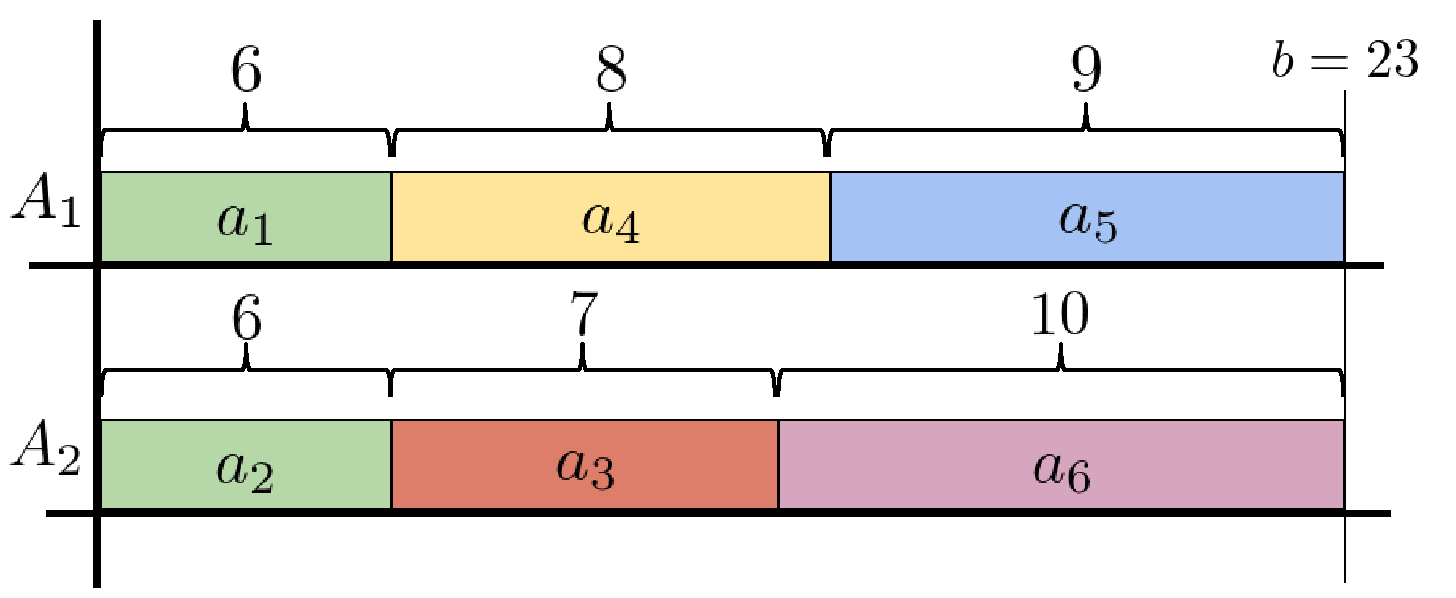
\includegraphics[width = 9cm]{figure/3-PARTITION.pdf}
  \caption{{\sc 3-PARTITION} の問題の解のイメージ}
\end{figure}

\textsc{3-SAT} と \textsc{3-PARTITION} の計算複雑さは NP 完全であることが Garey and Johnson [1990] \cite{3SAT} により証明されている.
ある決定問題が NP 完全であるとは,以下の二つが成立することを示す.
\begin{itemize}
  \item その問題が NP に属す.
  \item その問題が NP 困難である.
\end{itemize}
つまり,すべての NP である問題から還元でき,加えて, Yes となる証拠が
与えられた時その証拠が正しいことを多項式時間で確認できることを示す必要がある.
ただし全ての NP である問題は推移性が成り立つためどれか1つから還元する
ことが出来れば良い.

本研究では,\textsc{3-SAT} からの多項式時間還元により 無関連並列機械モデルにおいて,機械数が入力の一部の場合,最大待ち時間最小化問題が NP 完全であることを示す.
つまり,\textsc{3-SAT} のインスタンスから 最大待ち時間最小化問題 のインスタンスが
多項式時間で構成可能であり,加えて, \textsc{3-SAT}  の判定結果が Yes ならば
かつその場合に限り構成された  最大待ち時間最小化問題のインスタンスに対し判定結果が Yes であることを示す.加えて,スケジュールを証拠とし,最大待ち時間最小化問題 のインスタンスとスケジュールが与えられたとき,そのスケジュールにおける最大待ち時間が $w$ 以下を満たすかの判定が多項式時間で行えることを示すことにより,最大待ち時間最小化問題が NP 完全であることを示す.

%\begin{figure}[h]
%  \centering
\begin{center}
  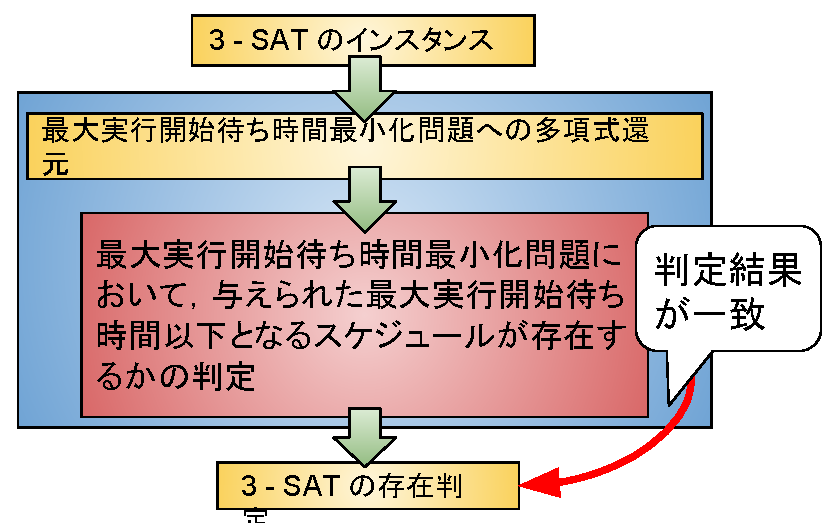
\includegraphics[width = 9cm]{figure/reduction.pdf}
\end{center}
%\end{figure}

この章では,最大待ち時間最小化問題を最適化問題,決定問題としてそれぞれ定義した.
また,最大待ち時間最小化問題と既存のスケジューリング問題の共通部分,差分をそれぞれまとめた.
次の章では,最大待ち時間最小化問題の関連問題である JIT ジョブ荷重和最大化問題と処理開始可能時刻付き最大遅れ時間最小化問題の従来研究の成果を紹介する.

\chapter{従来研究}\label{c_3}
第 \ref{c_3} 章では,従来研究の成果を紹介する.
第 \ref{3_s_1} 節では,JIT ジョブ荷重和最大化問題について,計算複雑さの観点から紹介する.
第 \ref{3_s_2} 節では,処理開始可能時刻付き最大遅れ時間最小化問題について,計算複雑さと解法の観点から紹介する.

\section{JITジョブ荷重和最大化問題}\label{3_s_1}
この問題は \textsc{3-SAT} からの還元により,強 NP 困難であることが Sung and Vlach \cite{SJIT} によって証明されている.以下では,JIT ジョブ荷重和最大化問題を定式化し,問題が NP 困難であることの証明を示す.
以下で,JIT ジョブ荷重和最大化問題の定式化を紹介する..
\begin{quote}
  \begin{description}
    \item[] {\bf JIT ジョブ荷重和最大化問題}
    \item[入力:] $n$ 個のジョブ $J_1,\ldots,J_n$ を $m$ 台の同一機械 $M_1,\ldots,M_m$
    で処理する.入力は,各 $i \in \{1,\ldots,n\}$ におけるジョブ $J_i$ の処理時
    間 $p_i$ ,処理開始可能時刻 $r_i$ ,納期 $d_i$ ,荷重 $w_i$ であり,
    それぞれの値は自然数である.
    各ジョブにおける処理時間の $n$ 次元ベクトル $P = (p_1,\ldots,p_n) \in \mathbb{N}^n$,
    処理開始可能時刻の $n$ 次元ベクトル $R = (r_1,\ldots,r_n) \in \mathbb{N}^n$ ,
    納期の $n$ 次元ベクトル $D = (d_1,\ldots,d_n) \in \mathbb{N}^n$ ,
    荷重の $n$ 次元ベクトル $W = (w_1,\ldots,w_n) \in \mathbb{N}^n$ からなる 4 項組 $(P,R,D,W)$.
    \item[解:] 問題の前提に基づき,スケジュールを定式化する.スケジュールは以下
    の条件を満たす $\forall j \in \{1,\ldots,m\}\big[A_j \subseteq
    \{1,\ldots,n\}\big]$ と $C : \{1,\ldots,n\} \to \mathbb{N}$ の対 $(A,
    C)$ であり,スケジュールによって,各ジョブを,どの機械で,いつ処理をするかを決める.
    \begin{itemize}
      \item $\forall i, i' \in \{1,\ldots,n\}\ \Big[ \big[i \neq i' \land A_i = A_{i'}\big] \Rightarrow$ \\ $~~~~~~~~~~~~~~~~~~~~~~~~~~~[C(i) - p_j, C(i)) \cap [C(i') - p_{i'}, C(i')) = \emptyset \Big]$
      \item  $\forall i \in \{1,\ldots,n\}\big[C(i) - p_i \ge r_i\big]$
    \end{itemize}
    \item[目的関数:] 実行可能なスケジュール $(A, C)$ のうち,納期以前に処理を完了するジョ
    ブの荷重和,
    \begin{displaymath}
      \displaystyle \varphi(A,C) = \sum_{i \in \mathcal{Q}(A,C)}w_i
    \end{displaymath}
    $i \in \mathcal{Q}(A,C)$ を最大とするスケジュールを求める.ただし,
    $\mathcal{Q}(A, C)$ はスケジュール $(A, C)$ に
    おいて納期以前に処理を完了するジョブの集合である (
    $\mathcal{Q}(A, C) = \{i \in \{1,\ldots, n\} | C(i) \ge d_i \}$ ).
  \end{description}
\end{quote}

以下では,\textsc{3-SAT} からの還元により,JIT ジョブ荷重和最大化問題の計算複雑さの証明を紹介する.

ブール型変数の集合 $X = \{x_1,\ldots,,x_β\}$ と, $X$ 上の 3 つのリテラル
からなる集合 $H = {h_1,\ldots,h_{\lambda}}$ の 2 項組, $(X,H)$ を任意の
\textsc{3-SAT} 問題の入力とする.
議論に先立ち,いくつかの表記を導入する.各 $k \in \{1,\ldots,\beta\}$
について, $\gamma_k$ を $H$ に おいて $x_k$ が現れる回数を表す自然
数とし, $\gamma$ を $\gamma_k ( k \in \{1,\ldots,\beta\} )$の最大値に
1 を加えた値とする($\displaystyle \gamma = \max_{k \in \{1,2,\ldots, \beta\}} \{\gamma_k \}+ 1$).
$(X, H)$ に基づき,以下のように JIT ジョブ荷重和最大化問題の入力
を設定する. $2\beta_{\gamma}$ 個のジョブを $\lambda + \beta$ 台の
無関連機械で処理する.各ジョブの処理時間,納期ズレ幅,納期,荷
重を以下のように設定する.

\begin{description}
  \item[納期ズレ幅の設定:]
  各ジョブ $i \in \{1,\ldots,2\beta \gamma\}$ の納期ズレ幅
  $\alpha_i$ を 0 とする.
  \item[納期の設定:] $\{1,2,\ldots, \beta \gamma\}$$ の $$\beta \gamma$ 個ジョブの納期につ
  いて,昇順で $\gamma$ 個ずつとった $\beta$ 個のグループについて,機械
  を順に対応させる.
  各グループ $k \in \{1,2,\ldots, \beta\}$ の $\gamma$ 番目のジョブの納
  期を $2\gamma - 1$,$\ell$ 番目のジョブ ( $\ell \neq \gamma$ ) の納期
  を $\ell$ とする.つまり,各 $k \in \{1,2,\ldots, \beta\}$ と $\ell \in \{1,2,\ldots,
  \gamma\}$について,
  \begin{displaymath}
    d_{(k - 1)\gamma + \ell} = \left\{ \begin{array}{ll} \ell & \text{if } \ell < \gamma \\ 2\gamma - 1 & \text{if } \ell = \gamma \end{array} \right.
  \end{displaymath}
  $\{\beta \gamma + 1,\ldots, 2\beta \gamma\}$ の $\beta \gamma$ 個のジョ
  ブの納期についても,同様に対応させる.
  各グループ $k \in \{1,2,\ldots, \beta\}$ の $\gamma$ 番目のジョブの納期を $\gamma$,$\ell$ 番目のジョブ ( $\ell \neq \gamma$ ) の納期を $\gamma + \ell$ とする.
  つまり,各 $k \in \{1,2,\ldots, \beta\}$ と $\ell \in \{1,2,\ldots,
  \gamma\}$について,
  \begin{displaymath}
    d_{(\beta + k - 1)\gamma + \ell} = \left\{ \begin{array}{ll}\gamma +  \ell & \text{if } \ell < \gamma \\ \gamma & \text{if } \ell = \gamma \end{array} \right.
  \end{displaymath}
  \item[荷重和の設定:] 各ジョブを納期昇順に基づき $2\beta$ 個のグループに分ける.
  グループ $k \in \{1,2,\ldots,\beta\}$ と,グループ $k + \beta$ について,グループの $\gamma$ 番目のジョブの荷重を $\gamma$ とし,それ以外のジョブの荷重を 1 とする.
  つまり,各 $k \in \{1,2,\ldots, \beta\}$ と $\ell \in \{1,2,\ldots,
  \gamma\}$について,
  \begin{displaymath}
    w_{(k - 1)\gamma + \ell^v} = w_{(\beta + k - 1)\gamma + \ell} = \left\{ \begin{array}{ll} 1 & \text{if } \ell < \gamma \\ \gamma & \text{if } \ell = \gamma \end{array} \right.
  \end{displaymath}
  \item[処理時間の設定:] 各ジョブを納期昇順に基づき $2\beta$ 個のグループに分ける
  グループ $k \in \{1,2,\ldots,\beta\}$ に機械を $k$ に対応させ,グルー
  プ $k + \beta$ にも同様に機械 $k$ を対応させる.各グループの各ジョブについて, グループに対応した機械以外の各機械における処理時間を $2\gamma$ とする.
  各グループの $\gamma$ 番目のジョブの,グループに対応する機械における処
  理時間を $\gamma$ とし,$\gamma$ 番目のジョブをのぞいた各ジョブの,グループに対応する機械における処理時間を 1 とする.
  つまり,各 $j \in \{1,2,\ldots, \beta\}$ と $k \in \{1,2,\ldots,
  \beta\}$ と $\ell \in \{1,2,\ldots, \gamma\}$について,
  \begin{displaymath}
    p_{(k - 1)\gamma + \ell, j} = p_{(\beta + k - 1)\gamma + \ell, j} = \left\{ \begin{array}{ll} 1 & \text{if } \ell < \gamma \text{ and } j = k, \\ \gamma & \text{if } \ell = \gamma \text{ and } j = k, \\ 2\gamma & \text{otherwise}\end{array} \right.
  \end{displaymath}

  残りの各機械 $j \in \{\beta + 1, \ldots , \beta + \gamma\}$ について,各ジョブの処理時間を設定する
  各グループ $k \in \{1,2,\ldots,\beta\}$ について,$x_k$ を対応させる.
  各グループ $k \in \{1,2,\ldots,\beta\}$ について,$\ell \in \{1,2,\ldots, \gamma - 1\}$ 番目の各ジョブにつ いて,$x_k \in h_{j - \beta}$ であれば $d_{(k - 1)\gamma + 1}$ とし,そうでない場合は $2\gamma$ とする.また,$\gamma$ 番目 のジョブの処理時間は $2\gamma$ とする.
  グループ $k + \beta$ について$\bar x_k$ を対応させる.
  $\ell \in \{1,2,\ldots, \gamma - 1\}$ 番目の各ジョブについて,$\bar x_k \in h_{j - \beta}$ であれば $d_{(\beta + k - 1)\gamma + \ell}$ とし, そうでない場合は $2\gamma$ とする.また,$\gamma$ 番目のジョブの処理時間は $2\gamma$ とする.
  つまり,各 $j \in \{\beta + 1,\ldots, \beta + \gamma\}$ と $k \in
  \{1,2,\ldots, \beta\}$ と $\ell \in \{1,2,\ldots, \gamma\}$について,
  \begin{displaymath}
    p_{(k - 1)\gamma + \ell, j} = \left\{ \begin{array}{ll} d_{(k - 1)\gamma + 1} & \text{if } \ell < \gamma \text{ and } x_k \in h_{j - \beta}, \\ 2\gamma & \text{otherwise} \end{array} \right.
  \end{displaymath}
  \begin{displaymath}
    p_{(\beta + k - 1)\gamma + \ell, j} = \left\{ \begin{array}{ll} d_{(\beta + k - 1)\gamma + \ell} & \text{if } \ell < \gamma \text{ and } \bar x_k \in h_{j - \beta}, \\ 2\gamma & \text{otherwise} \end{array} \right.
  \end{displaymath}
\end{description}

このように設定した $(P,a,D,W)$ は JIT ジョブ荷重和最大化問題の入力である.以降,$(X,H)$ に基づいて前述のように設定した $(P,a,D,W)$ を区別して $I_{(X,H)}$ と表す $(I_{(X,H)} = (P,a,D,W))$.
以下,$H$ を充足する真理値割り当て $f : X \to \{0,1\}$ が存在すること
と,$I_{(X,H)}$ を入力とする JIT ジョブ荷重和最大化問題に対して
$\varphi(A,C) \ge \beta(2\gamma - 1) + \lambda$ を満たす実行可能なスケ
ジュール $(A,C)$ が存在することが,同値であることを示す.

\begin{lemma}\label{l_1}
  $H$ を充足する真理値割り当て $f : X \to \{0,1\}$ が存在するならば,$I_{(X,H)}$ を入力とする JIT ジョブ荷重和最大化問題に対して
  $\varphi(A, C) \ge \beta(2\gamma - 1) + \lambda$ を満たす実行可能なス
  ケジュール $(A, C)$ が存在する.
\end{lemma}

\begin{proof}
  $(X,H)$ を任意の 3 -SAT 問題の入力とし, $f : X \to \{0,1\}$ を $H$ を
  充足する真理値割り当てとする.つまり, $f$ は以下を満たす.
  \begin{displaymath}
    \displaystyle \bigwedge_{h \in H} \bigg(\bigvee_{x \in h}f(x) \lor
    \bigvee_{\bar x \in h}\lnot f(x) \bigg) = 1
  \end{displaymath}
  各 $k \in \{1,\ldots, \beta\}$ について, $f(x_k) = 1$ ならばグルー
  プ $\beta + k$ の全てのジョブを,グループ $\beta + k$ に対応する機械
  $k$ に割り当て,そうでなければグルー
  プ $k$ の全てのジョ ブを,グループ $k$ に対応する機械 $k$ に割り当てる.ま
  た,機械 $k$ に割り当てた各ジョ ブの完了時刻を納期とする.つまり,
  $f(x_k) = 1$ ならば,各 $\ell \in \{1,\ldots,\gamma\}$ について $A_k
  :=A_k cup\{(\beta+k−1)\gamma+\ell\}$ かつ
  $C((\beta+k−1)\gamma+\ell)=d(\beta+k−1)\gamma+l$ ,$f(x_k)=0$ なら
  ば,各 $\ell \in \{1,\ldots,\gamma \}$ について$A_k :=A_k \cup
  \{(k−1)\gamma+\ell \}$ かつ $C((k−1)\gamma+\ell)=d(k−1)\gamma+\ell$
  . $I_{(X,H)}$ の定義より,ここまでのスケジュールにおいて,機械
  $1,\ldots, \beta$ に割り当てたジョ ブの処理時間は重複せず (図 3.1),完
  了時刻は納期であることから,$k \in \{1,\ldots,\beta\}$ に割り当てたジョ
  ブは JIT ジョブである.よって,ここまでのスケジュール $(A, C)$ における
  JIT ジョブの荷重和は,
  \begin{displaymath}
    \displaystyle \varphi(A,C) = \sum_{k \in
    \{1,\ldots,\beta\}}\bigg(\sum_{i \in \mathcal{Q}(A,C):i \in
    A_k}w_i\bigg) = \sum_{k \in \{1,\ldots,\beta\}}(2\gamma - 1) =
    \beta(2\gamma - 1)
  \end{displaymath}

  \begin{figure}[h]
    \centering
    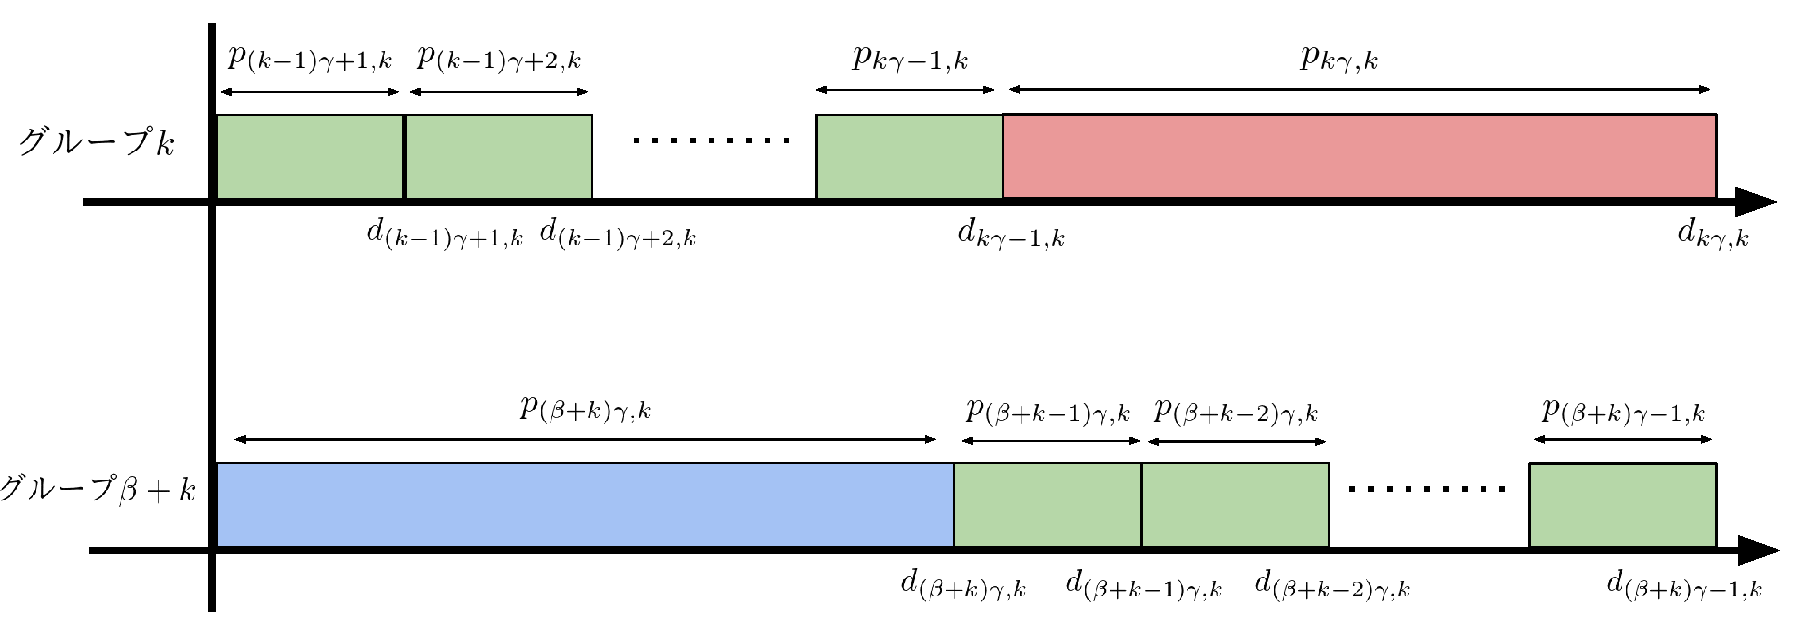
\includegraphics[width = 15cm]{figure/SJIT.pdf}
    \caption{機械 $k \in \{1,\ldots,\beta\}$ に対応するグループ $k$
    とグループ $\beta + k$ の各ジョブ}
  \end{figure}

  各 $j\in \{1,\ldots,\lambda\}$ について,$f(x_k)=1$ を満たす$x_k \in
  h_j$ か,$f(x_k)=0$ を満たす $\bar x_k \in h_j$ をひとつ見つける. $f$ が $H$ を充足することから,各 $j \in \{1,\ldots,\lambda\}$ について, 上記を満たすリテラルは必ず存在する.
  与えられた $j \in \{1,\ldots,\lambda \}$ について, $f(x_k) = 1$ を満
  たす $x_k \in h_j$ を見つけたと仮定す る.グループ $k$ のジョブ
  のうち,いずれの機械にも割り当てられていない $\ell \in
  \{1,\ldots,\gamma - 1\}$ を見つける.グループ $k$ のジョブは,
  $f (x_k) = 1$ であることから,$\{1,\ldots, \beta \}$ のいずれの機
  械にも割り当てられておらず,また,各リテラルが現れる回数は高々
  $\gamma − 1$ であることから,そのような $\ell$ 番目のジョブは必す
  ゙存在する. $A_{j + \beta} := A_{j + \beta} \cup \{ (k − 1) \gamma +
  \ell\}$ とし, $C((k − 1)\gamma + l) = d(k−1)\gamma + \ell$ とする.
  次に,与えられた $j \in \{1,\ldots,\lambda\}$ について, $f(x_k) = 0$
  を満たす $\bar x_k \in h_j$ を見つけたと仮定する.グループ $\beta
  + k$ のジョブのうち,いずれの機械にも割り当てられていない $\ell
  \in \{1,\ldots,\gamma\}$ を見つける.先ほどと同様の議論で,そのよ
  うな $\ell$ は必ず存在する. $A_{j + \beta} := A_{j + \beta} \cup \{
  (\beta + k − 1 ) \gamma + \ell \} = j + \beta$ とし,$C((\beta + k −
  1) \gamma + \ell) = d(\beta + k − 1)\gamma + \ell$ とする.
  各グループの $\ell \in \{1,\ldots,\gamma − 1\}$ 番目のジョブ
  の荷重が 1 であることから,各 $j \in \{1,\ldots, \lambda \}$ につ
  いて $j$ に割り当てられた JIT ジョブの荷重和は,
  $$\displaystyle \sum_{i \in \mathcal{Q}(A,C):A(i) = j + \beta}w_i =
  1$$
  ここまでのスケジュール $(A, C)$ においていずれの機械にも割り当てられて
  いないジョブを, $\max\{d_i | i \in \{1,\ldots, 2\beta \gamma\}$ のあと,任意の順,任意の機械で処理するものとする.
  明らかにスケジュール $(A, C)$ は実行可能であり,以下を満たす.
  \begin{displaymath}
    \displaystyle \varphi(A,C) = \sum_{j \in
    \{1,\ldots,\beta\}} \sum_{i \in \mathcal{Q}(A,C):i \in
    A_j}w_i + \sum_{j \in
    \{\beta + 1,\ldots,\lambda + \beta\}} \sum_{i \in \mathcal{Q}(A,C):i \in
    A_j}w_i =
    \beta(2\gamma - 1) + \lambda
  \end{displaymath}
\end{proof}

ここで, $I_{(X,H)}$ を入力とする JIT ジョブ荷重和最大化問題に
おける実行可能なスケジュールについて,いくつかの性質を示す.
$(A, C)$ を $_{I(X,H)}$ を入力とする JIT ジョブ荷重和最大化問題に
おける任意の実行可能なスケジュールとする.実行可能性の制約により,各シ
゙ョブは機械の稼働開始時刻以降に処理を開始することから,各 JIT ジョ
ブ $i \in \mathcal{Q}(A,C)$ について,$C(i) − p_i = d_i − p_i \ge 0$ であ
る.このことから,$p_i,j \ge 2\gamma$ かつ $d_i \le 2\gamma − 1$ を満
たす $i \in \{1,\ldots,n\}$ と $j \in \{1,\ldots,m\}$ について,$i \in
\mathcal{Q}(A,C)$ のとき,$i \notin A_j$ である.したがって,
$I_{(X,H)}$ の定義より,各 $k \in \{1,\ldots,\beta\}$ について,
\begin{itemize}
  \item $i \in \mathcal{Q}(A,C)$ かつ $i \in A_k$ ならば,
  $(k − 1)\gamma + 1 \le i \le k\gamma$ または $(\beta + k − 1)\gamma +
  1 \le i \le (\beta + k)\gamma$ である.
  \item $k\gamma \in \mathcal{Q}(A,C)$ ならば $k\gamma \in A_k$ であ
  り,$\beta + k)\gamma \in \mathcal{Q}(A,C)$ な
  らば $(\beta + k)\gamma \in A_k$ である.
\end{itemize}
実行可能性の制約より,同じ機械に割り当てられた複数のジョブの処理
は重複しないこと から,各 $k \in \{1,\ldots,\beta\}$ について,
\begin{itemize}
  \item $k\gamma \in \mathcal{Q}(A,C)$ ならば,$i \in A_k$ である任
  意の $i \in \mathcal{Q}(A,C)$ について,$i$ は \\$(k − 1)\gamma− 1
  \le k\gamma$ を満たす (図 $3.1$).
  \item $(\beta + k)\gamma \in \mathcal{Q}(A,C)$ ならば,$i \in A_k$ て
  ゙ある任意の $i \in \mathcal{Q}(A,C)$ について,$i$ は
  $(\beta + k − 1)\gamma − 1 \le i \le (\beta + k)\gamma$ を満たす.
\end{itemize}
以上の議論より,各 $k \in \{1,\ldots, \beta \}$ について,$k$ に割り当
てられた JIT ジョブの荷重和は以下を満たし
\begin{equation}
  \sum_{i \in \mathcal{Q}(A,C):i \in A_k}w_i \le
  2\gamma - 1 \tag{A.1}
\end{equation}

% タグづけがまだできていない
以下のいずれかを満たす場合にのみ,$\displaystyle \sum_{i \in \mathcal{Q}(A,C):i \in A_k}w_i = 2\gamma - 1$ となる.
\begin{equation}
  \{i \in \mathcal{Q}(A,C) \mid i \in A_k\} = \{(k - 1)\gamma + 1, (k
  - 1)\gamma + 2,\ldots,k\gamma\} \tag{A.2}
\end{equation}
\begin{equation}
  \{i \in \mathcal{Q}(A,C) \mid i \in A_k\} = \{(\beta + k -
  1)\gamma + 1, (\beta + k
  - 1)\gamma + 2,\ldots,(\beta + k)\gamma\} \tag{A.3}
\end{equation}
さらに,各 $j \in \{\beta + 1,\ldots, \beta + \lambda \}$ について,
各ジョブ $i \in \{1,\ldots, 2\beta \gamma \}$ の処理時間は $p_ij
\in \{d_i, 2\gamma \}$ であり,機械 $j$ に割り当てられるジョブは
高々 1 つである ( $|\{i \in \mathcal{Q}(A, C)\} | i \in A_j \}| \le 1$
).既に述べたように,各 $k \in \{1,\ldots,\beta \}$ について
$k\gamma \in \mathcal{Q}(A,C)$ ならば $k\gamma \in A_k$ であり,
$(\beta + k) \gamma \in \mathcal{Q}(A,C)$ ならば,$(\beta +
k)\gamma \in A_k$ である.これらのジョブをのぞいた各ジョブの荷
重は 1 であることから,各 $j \in \{ \beta + 1,\ldots,
\lambda + \beta \}$ について,
\begin{equation}
  \displaystyle \sum_{i \in \mathcal{Q}:i \in A_j}w_i \le 1 \tag{A.4}
\end{equation}

\begin{lemma}\label{l_2}
  $I_{(X,H)}$ を入力とする JIT ジョブ荷重和最大化問題に対して
  $\varphi(A, C) \ge \beta(2\gamma − 1) + \lambda$ を満たす実行可能なス
  ケジュール $(A, C)$ が存在するならば,$H$ を充足する真理値割り当
  て $f : X \to \{0, 1\}$ が存在する.
\end{lemma}

\begin{proof}
  $(A, C)$ を $I_{(X,H)}$ を入力とする JIT ジョブ荷重和最大化問題に
  対して $\varphi(A, C) \ge \beta (2\gamma − 1) + \lambda$ を満たす実行
  可能なスケジュールとする.式 ($15$) と式 ($A.4$) より $\varphi(A, C
  )\le≤ \beta(2\gamma − 1) + \lambda$ であり,このことから,
  $\varphi(A, C) = \beta (2\gamma − 1) + \lambda$ である.
  各機械 $k \in \{1,\ldots, \beta\}$ について,式 ($A.2$) または式
  ($A.3$) が満たされ,各 $j \in \{ \beta + 1,\ldots,\beta + \lambda
  \}$ について,$|\{ i \in \mathcal{Q}(A,C) | i \in A_j \} | = 1$ で
  ある.$(A,C)$ に基づき,$f : H \to \{0,1\}$ を以下のように設定する.
  各 $k \in \{1,\ldots, \beta \}$ について,式 ($A.3$) が満たされる
  ならば $f(x_k) = 1$ とし,そうでなければ $f(x_k) = 0$ とする.
  明らかに,各 $j \in \{\beta + 1,\ldots,\beta + \lambda \}$ について
  $j$ に割り当てられたただ一つの JIT ジョブ $i \in
  \mathcal{Q}(A,C)$ が存在し,$i \ge \beta \gamma$ ならば $f(x_k)
  = 1$ を満たすある $x_k \in h_{j - \beta}$ が存在し,$i > \beta
  \gamma$ ならば $f(x_k) = 0$ を満たすある $\bar x_k \in h_{j -
  \beta}$ が存在する.したがって,$f$ は $H$ を充足する真理値割り当てである.
\end{proof}

補題 \ref{l_1} と補題 \ref{l_2} より,$H$ を充足する真理値割り当て $f : X \to \{0,
1\}$ が存在することと,$I_{(X,H)}$ を入力とする JIT ジョブ荷重和
最大化問題に対して $\varphi(A, C) \ge \beta(2\gamma − 1) + \lambda$
を満たす実行可能なスケジュール $(A, C)$ が存在することは,同値で
ある.
3 -SAT 問題の入力 $(X,H)$ に基づく $I_{(X,H)}$ の生成に要する計算時
間は,明らかに多項式時間であり,入力 $I_{(X,H)}$ の長さは,$(X, H)$
の長さに関する多項式で表すことができる.したがって,無関連並列
機械モデルにおいて機械数が入力の一部の場合, JIT ジョブ荷重和
最大化問題は強 NP 困難である.

\section{処理開始可能時刻付き最大遅れ時間最小化問題}\label{3_s_2}

この問題は \textsc{3-PARTITION} からの還元により,強 NP 困難であることが Garey and Johnson \cite{3SAT}によって,証明されている.
以下では,処理開始可能時刻付き最大遅れ時間最小化問題を定式化し,問題が NP 困難であることの証明を示す.
以下では,処理開始可能時刻付き最大遅れ時間最小化問題の定式化を紹介する.
\begin{quote}
  \begin{description}
    \item[] {\bf 処理開始可能時刻付き最大遅れ時間最小化問題}
    \item[入力:] $n$ 個のジョブ $J_1,\ldots,J_n$ を 1 台の機械で処理する.入力は,各 $i \in \{1,\ldots,n\}$ におけるジョブ $J_i$ の処理時間 $p_i$,処理開始可能時刻
    $r_i$,納期 $d_i$ であり,それぞれの値は自然数である.各ジョブにおける処理時間の $n$ 次元ベクトル $P = (p_1,\ldots,p_n) \in \mathbb{N}^n$ ,
    処理開始可能時刻の $n$ 次元ベクトル $R = (r_1,\ldots,r_n) \in \mathbb{N}^n$ ,
    納期の $n$ 次元ベクトル $D = (d_1,\ldots,d_n) \in \mathbb{N}^n$ からなる 3項組 $(P,R,D)$.
    \item[解:] 問題の前提に基づき,スケジュールを定式化する.スケジュールは以下
    の条件を満たす $C : \{1,\ldots,n\} \to \mathbb{N}$ であり,スケジュー
    ルによって,各ジョブ,をいつ処理をするかを決める.
    \begin{itemize}
      \item $\forall i, i' \in \{1,\ldots,n\}\ \Big[ \big[i \neq i' \big] \Rightarrow$ \\ $~~~~~~~~~~~~~~~~~~~~~~~~~~[C(i) - p_i, C(i)) \cap [C(i') - p_{i'}, C(i')) = \emptyset \Big]$
      \begin{itemize}
        \item 機械は同時に複数のジョブを処理しない
        \item 各ジョブの処理を開始すると,完了するまで中断しない
      \end{itemize}
      \item  $\forall i \in \{1,\ldots,n\}\big[C(i) - p_i \ge r_i\big]$
      \begin{itemize}
        \item 各ジョブは処理開始可能時刻以降によりを開始する
      \end{itemize}
    \end{itemize}
    \item[目的関数:] 実行可能なスケジュール $C$ のうち,最大の納期遅れ,
    \begin{displaymath}
      \varphi(C) = \max_{i \in \{1,\ldots,n\}}\{C(i) - d_i\}
    \end{displaymath}
    を最小とするスケジュールを求める.
  \end{description}
\end{quote}

以下では,\textsc{3-PARTITION} からの還元により,処理開始可能時刻つき最大遅れ時間最小化問題の計算複雑さを証明を紹介する.

整数の集合 $S = \{a_1,\ldots,a_{3t}\}$ と 整数 $b$ の 2 項組 $(S,b)$ を \textsc{3-PARTITION} の
任意の入力とする.$(S,a)$ に基づき,以下のように最大遅れ時間最小化問題
の入力を設定する.$4t - 1$ 個のジョブを 1 台の機械で処理する.各゙ジョ
ブの処理時間,納期ズレ幅,納期を以下のように設定する.

集合 $S$ の冪集合の部分集合 $\mathcal{A} \subseteq 2^{S}$ が以下を満たすとき,{\sc 3-PARTITION} の解は Yes.
\begin{itemize}
  \item $\forall A \in \mathcal{A}[|A| = 3 \land \sum_{a \in A} a = b]$
  \item $\bigcup_{A \in \mathcal{A}} A = S$
  \item $\forall A, A' \in \mathcal{A}[A \neq A' \Rightarrow A \cap A' = \emptyset]$
\end{itemize}

\begin{description}
  \item[処理時間開始可能時刻の設定:] 各 $i \in \{1,\ldots,4t - 1\}$ におけるジョブ $J_i$ の処理開始可能時刻について,$1 \le i \le t - 1$ のとき,$r_i = ib + (i - 1)$,$t \le i \le 4t - 1$ のとき,$r_{i} = 0$ とする.
\end{description}
\begin{displaymath}
  r_i = \left\{ \begin{array}{ll} ib + (i - 1) & \text{if } 1 \le i \le t - 1 \\ 0 & \text{if } t \le i \le 4t - 1\end{array} \right.
\end{displaymath}
\begin{description}
  \item[処理時間の設定:] 各 $i \in \{1,\ldots,4t - 1\}$ におけるジョブ $J_i$ の処理時間について,$1 \le i \le t - 1$ のとき,$p_i = 1$,$t \le i \le 4t - 1$ のとき,$p_{i} = a_{i - t + 1}$ とする.
\end{description}
\begin{displaymath}
  p_i = \left\{ \begin{array}{ll} 1 & \text{if } 1 \le i \le t - 1 \\ a_{i - t + 1} & \text{if } t \le i \le 4t - 1\end{array} \right.
\end{displaymath}
\begin{description}
  \item[納期の設定:] 各 $i \in \{1,\ldots,4t - 1\}$ におけるジョブ $J_i$ の処理時間について,$1 \le i \le t - 1$ のとき,$d_i = ib + i$,$t \le i \le 4t - 1$ のとき,$d_i = tb + (t - 1)$ とする.
\end{description}
\begin{displaymath}
  d_i = \left\{ \begin{array}{ll} ib + i & \text{if } 1 \le i \le t - 1 \\ tb + (t - 1) & \text{if } t \le i \le 4t - 1\end{array} \right.
\end{displaymath}

このように設定した $(P,R,D)$ は最大遅れ時間最小化問題の入力である.以
降,$(S,b)$ に基づいて前述のように設定した $(P,R,D)$ を区別して
$I_{(S,b)}$ と表す.以下,上記の条件を満たす$\mathcal{A} \subseteq 2^S$ が存在
することと,$I_{(S,b)}$ を入力とする最大遅れ時間最小化問題に対して
$\varphi(C) =  0$
を満たす実行可能なスケジュール $C$ が存在することは,同値で
あることを示す.
\begin{lemma}\label{l_3}
  上記の条件を満たす $\mathcal{A} \subseteq 2^S$ が存在するならば,
  $I_{(S,b)}$ を入力とする最大遅れ時間最小化問題に対して $\varphi(C) =
  0$ を満たす実行可能なスケジュール $C$ が存在する.
\end{lemma}

\begin{proof}
  各 $1 \le i \le t - 1$ におけるジョブ $J_i$ を機械に割り当てる.各 $1 \le i \le t - 1$ におけるジョブ $J_i$ の処理時間は 1 であることから,$[0, tb + (t - 1)]$ の区間は,$t - 1$ 個のジョブによって,$t$ 個区間に分断され,それぞれの長さは $b$ である.
  (図 3.2)
  \begin{figure}[h]
    \centering
    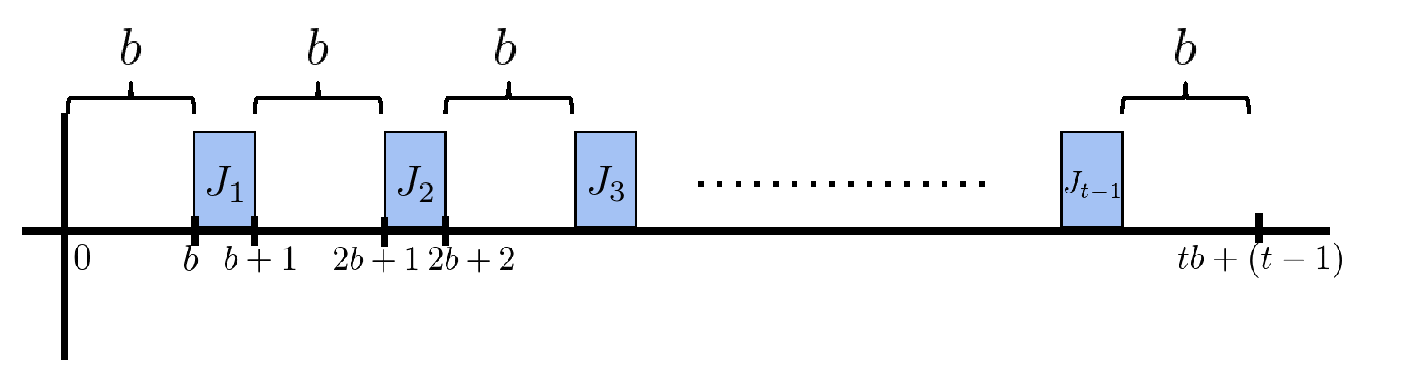
\includegraphics[width = 14cm]{figure/Lmax.pdf}
    \caption{各 $1 \le i \le t - 1$ におけるジョブ $J_i$ の配置による区間の分割}
  \end{figure}

  ここで,上記の条件を満たす $\mathcal{A} \subseteq 2^S$ が存在す
  ることから,$\forall A \in \mathcal{A}\big[|A| = 3 \land \sum_{a \in
  A}a = b \big]$ である.このとき,各 $t \le i \le 4t - 1$ におけるジョブ $J_{i}$ は 長さ $b$ の $t$ 個の区間のいずれかに割り当てられる.また,各区間に割り当てられた 3 つのジョブの処理時間の和は$I_{(S,b)}$ より,$b$ である.

  以上より,上記の条件を満たす $\mathcal{A} \subseteq 2^S$ が存在するならば,
  $I_{(S,b)}$ を入力とする最大遅れ時間最小化問題に対して $\varphi(C) =
  0$ を満たす実行可能なスケジュール $C$ が存在する.
\end{proof}

\begin{lemma}\label{l_4}
  上記の条件を満たす $\mathcal{A} \subseteq 2^S$ が存在しないならば,$I_{(S,b)}$ を入力とする最大遅れ時間最小化問題に対して $\varphi(C) \le
  0$ を満たす実行可能なスケジュール $C$ が存在しない.
\end{lemma}

\begin{proof}
  各 $1 \le i \le t - 1$ におけるジョブ $J_i$ を機械に割り当てる.各 $1 \le i \le t - 1$ におけるジョブ $J_i$ の処理時間は 1 であることから,$[0, tb + (t - 1)]$ の区間は,$t - 1$ 個のジョブによって,$t$ 個区間に分断され,それぞれの長さは $b$ である.
  (図 3.2)

  ここで,上記の条件を満たす $\mathcal{A} \subseteq 2^S$ が存在し
  ないことから,$\forall A \in \mathcal{A}\big[|A| = 3 \land \sum_{a \in
  A}a \neq b \big]$ である.これより,各 $t \le i \le 4t - 1$ に
  おけるジョブ $J_{i}$ は 長さ $b$ の $t$ 個の区間のいずれかに割り当てるとき,各区間のジョブの処理時間の和が $b$ でない区間が少なくとも 1 つ存在する.以上より,上記の条件を満たす $\mathcal{A} \subseteq 2^S$ が存在しないならば,$I_{(S,b)}$ を入力とする最大遅れ時間最小化問題に対して$\varphi(C) = 0$ を満たす実行可能なスケジュール $C$ は存在しない.
\end{proof}

補題~\ref{l_3} と補題~\ref{l_4} より,上記の条件を満たす$\mathcal{A} \subseteq 2^S$ が存在
することと,$I_{(S,b)}$ を入力とする最大遅れ時間最小化問題に対して
$\varphi(C) \le  0$
を満たす実行可能なスケジュール $C$ が存在することは,同値で
ある.
3 -PARTITION 問題の入力 $(S,b)$ に基づく $I_{(S,b)}$ の生成に要する計算時
間は,明らかに多項式時間であり,入力 $I_{(S,b)}$ の長さは,$(S, b)$
の長さに関する多項式で表すことができる.したがって,単一
機械モデルにおいて,最大遅れ時間最小化問題は強 NP 困難である.


処理開始可能時刻付き最大遅れ時間最小化問題は,各制約により制限を加えることで多項
式時間で最適解が求まることが Lawler \cite{EDD1},Lageweg, Lenstra, and Rinnooy Kan \cite{EDD2} によって証明されている.各部分問題に対する解法は以下の通り.

\begin{itemize}
  \item \textbf{処理開始可能時刻の制約に対する制限}:$\forall j \in \{1,\ldots,n\}\big[ r_j = r \big]$

  ジョブを納期の昇順で処理する( EDD ルール ) .このとき,スケジュールにおける任意の 2 つのジョブは以下の条件を満たす.
  \begin{displaymath}
    \forall i, j \in \{1,\ldots,n\}\big[d_i \le d_j \Rightarrow C(i) \le C(j)\big]
  \end{displaymath}
  \item \textbf{処理時間の制約に対する制限}:$\forall j \in \{1,\ldots,n\}\big[ p_j = p \big]$

  スケジュール可能なジョブの中で,納期が最も小さいジョブ順に処理する.このとき,スケジュールにおける各ジョブを順に $J_1,\ldots,J_n$,$C(0) = 0$ とすると,各ジョブは以下の条件を満たす.
  \begin{displaymath}
    \forall j, j' \in \bigg\{i \mid \forall i \in \{1,\ldots,n\}\big[r_i \le C(i - 1)\big]\bigg\}\bigg[j \le j' \Rightarrow d_j \le d_j'\bigg]
  \end{displaymath}
  \item \textbf{納期の制約に対する制限}:$\forall j \in \{1,\ldots,n\}\big[ d_j = d \big]$

  ジョブを処理開始可能時刻の昇順で処理する.このとき,スケジュールにおける任意の 2 つのジョブは以下の条件を満たす.
  \begin{displaymath}
    \forall i, j \in \{1,\ldots,n\}\big[r_i \le r_j \Rightarrow C(i) \le C(j)\big]
  \end{displaymath}
\end{itemize}

ここで,処理開始可能時刻を一定とした最大遅れ時間最小化問題の部分問題に対して,EDD ルールを適用することで最適解が求まることの証明を示す.

\begin{lemma}\label{l_5}
  処理開始可能時刻を一定とした最大遅れ時間最小化問題の部分問題に対して,EDD ルールを適用することで最適解が求まる.
\end{lemma}

\begin{proof}
  スケジュール $S$ をある 2 つの連続するジョブ $J_i$, $J_k$ について納期順に並んでいないジョブを含むスケジュールとし,$S'$ を納期の昇順で並んでいるスケジュールとする.
  ただし,全てのジョブの処理時間は 0 以上とする.
  つまり,スケジュール $S$ におけるジョブ $J_i$,$J_k$ の納期は,$d_i > d_k$ であり,スケジュール $S'$ におけるジョブ $J_i$,$J_k$ の納期は,$d_i < d_k$ である.
  上記の条件をまとめた図は以下の通りである.(図 3.3)

  \begin{figure}[h]
    \centering
    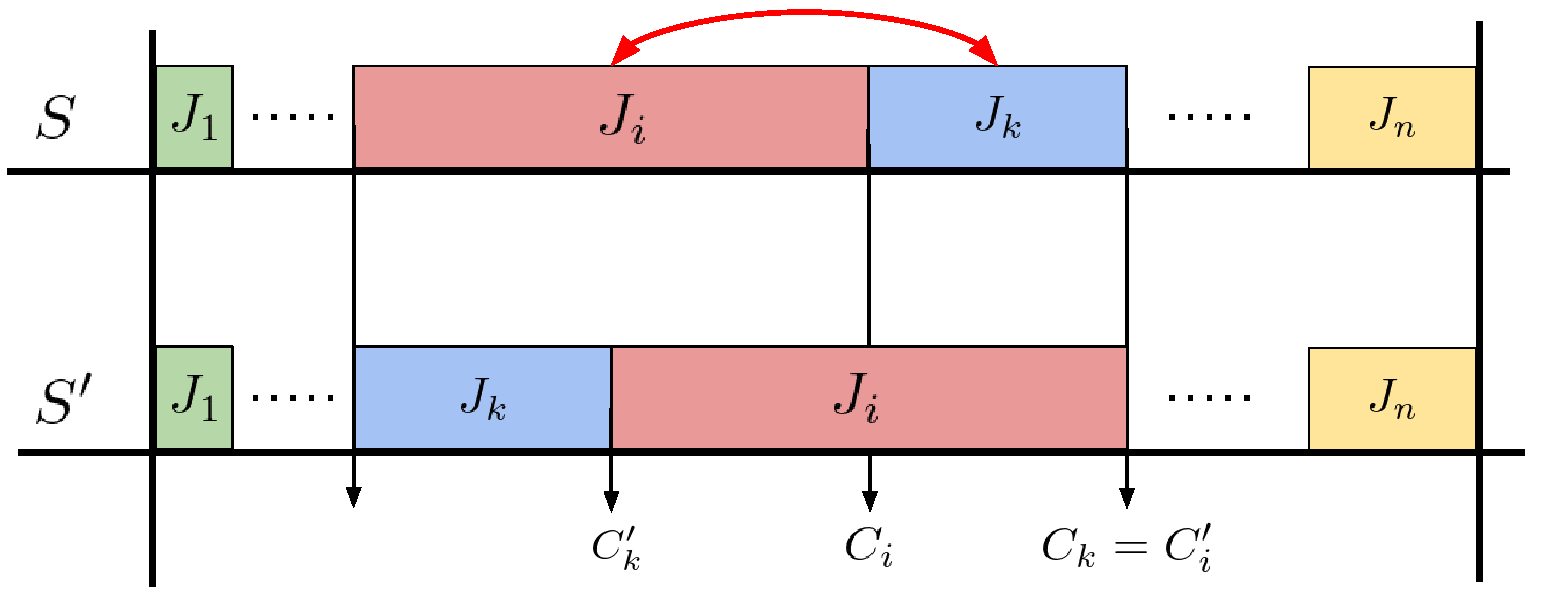
\includegraphics[width = 11cm]{figure/EDDrule.pdf}
    \caption{納期順に割り当てられていないスケジュール $S$ と納期順に割り当てられたスケジュール $S'$}
  \end{figure}

  前提より,すべてのジョブの処理開始可能時刻が等しいことから,スケジュール $S$ における,ジョブ $J_i$ の処理開始時刻とスケジュール $S'$ におけるジョブ $J_k$ の処理開始時刻は等しい.つまり,$C_i - p_i = C'_k - p_k$ である.
  同様に,スケジュール $S$ における,ジョブ $J_k$ の完了時刻とスケジュール $S'$ におけるジョブ $J_i$ の完了時刻は等しい.つまり,$C_k = C'_i$ である.
  以上より,
  スケジュール $S$ におけるジョブ $J_i$ の遅れ時間 $L_i(S)$ は,$L_i(S) = C_i - d_i$,ジョブ $J_k$ の遅れ時間 $L_k(S)$ は $L_k(S) = C_k - d_k$ となる.
  同様に,スケジュール $S'$ におけるジョブ $J_i$ の遅れ時間 $L_i(S')$ は,$L_i(S') = C'_i - d_i = C_k - d_i \le C_k - d_k = L_k(S)$,ジョブ $J_k$ の遅れ時間 $L_k(S')$ は,$L_k(S') = C'_k - d_k \le C_k - d_k = L_k(S)$ と表すことができる.
  ここで,ジョブ $J_i,\ J_k$ を除いたジョブにおける最大遅れ時間を $L(S)$
  とする.つまり,$L(S) = \displaystyle \max_{j \in \{1,\ldots,n\}
  \setminus \{i,k\}}L_j(S)$.よって,スケジュール $S$,スケジュール
  $S'$ における最大遅れ時間はそれぞれ,次のように表すことができる.
  \begin{displaymath}
    \left\{ \begin{array}{lll} L_{\max}(S) =
    \max\bigg\{L(S),L_i(S),L_k(S)\bigg\} \\ L_{\max}(S') =
    \max\bigg\{L(S),L_i(S'),L_k(S')\bigg\}\end{array} \right.
  \end{displaymath}

  今までの議論より,$L_{\max}(S') \le L_{\max}(S)$ であることは明らかで
  ある.

  ここで,スケジュールの全体集合を $\mathcal{S}$,EDD ルールを適用したスケ
  ジュールの集合を $\mathcal{S}'$ とすると,
  前述の議論より,$\forall S \in \mathcal{S}$, $\exists S' \in \mathcal{S}'$, $L_{\max}(S') \le L_{\max}(S)$ と表すことができる.また,どのスケジュールに対しても,
  EDD ルールを適用することで,一つの解に収束するので,
  $\forall S, S' \in \mathcal{S}'$, $L_{\max}(S) = L_{\max}(S')$ と表す
  ことできる.
  以上より,$\forall S \in \mathcal{S}$, $\forall
  S' \in \mathcal{S}'$, $L_{\max}(S') \le L_{\max}(S)$ となる.
\end{proof}

補題~\ref{l_5} より,処理開始可能時刻を一定とした最大遅れ時間最小化問題の部分問題に対して,EDD ルールを適用することで最適解が求まることを示せた.

全てのジョブにおける処理時間や納期が常に一定であるときも,同様に証明で
きる.以降,これらの証明と解法に着目して,最大待ち時間最小化問題の計算複雑さの証明,解法の提案を行う.

\chapter{最大待ち時間最小化問題の計算複雑さ}\label{c_4}
最大待ち時間最小化問題は,どの機械モデルにおいても,計算複雑さ
が明らかでない.第 \ref{4_s_1} 節では,無関連並列機械モデルにおける最大待ち時間最小化問題の NP 完全性の証明を行う.第 \ref{4_s_2} 節では,最大待ち時間最小化問題の計算複雑さについてまとめる.

\section{無関連並列機械モデルにおける NP 完全性の証明}\label{4_s_1}
以下は,最大待ち時間最小化問題を $w$ 以下となるスケジュールが存在するかという決定問題として定式化した待ち時間制約付きスケジューリング問題に対する証明である.

ブール型変数の集合 $X =\{x_1, x_2,\ldots ,x_n\}$ と, $X$ 上の 3 つのリテラルからなる集合の集合 $H =\{h_1, h_2,\ldots ,h_{\lambda}\}$ の 2 項組,$(X,H)$ を任意の \textsc{3-SAT} 問題の入力とする.

各 $i \in \{1,2,\ldots, n\}$ について,$\alpha_i$ を $H$ に おいて $x_i$ が現れる回数を表す自然数とし,$\beta_i$ を $H$ において $\bar x_i$ が現れる回数を表す自然数とする.
つまり,$\alpha_i = \big|\{h \in H \mid x_i \in h\}\big|$,$\beta_i = \big|\{h \in H \mid \bar x_i \in h\}\big|$
また,$\displaystyle \sum_{i \in \{1,\ldots,n\}} \alpha_i = \mathcal{A}$, $\displaystyle \sum_{i \in \{1,\ldots,n\}} \beta_i = \mathcal{B}$  とする.

ただし,各 $i \in \{1,2,\ldots, n\}$ について,$\alpha_i$, $\beta_i$ は 3 以上とする.\\
つまり,$\forall i \in \{1,\ldots,n\}\big[\alpha_i \ge 3\big]$,
$\forall i \in \{1,\ldots,n\}\big[\beta_i \ge 3\big]$

$(X.H)$ に基づき,以下のように待ち時間制約付きスケジューリング問題の入力を設定する.
$2(\mathcal{A} + \mathcal{B}) + \lambda$ 個のジョブ $\mathcal{J}$ を
$n + \lambda$ 台の無関連機械 $\mathcal{M}$ で処理する.
\begin{itemize}
  \item $\mathcal{J}^t \subset \mathcal{J}$ s.t. $|\mathcal{J}^t| =
  \mathcal{A}  + \mathcal{B}$,
  \item $\mathcal{J}^f \subset \mathcal{J}$
  s.t.$|\mathcal{J}^f| = \mathcal{A}  + \mathcal{B}$,
  \item $\mathcal{J}^d \subset \mathcal{J}$ s.t.$|\mathcal{J}^d| =
  \lambda$
\end{itemize}
ただし,$\mathcal{J} = \mathcal{J}^t \cup \mathcal{J}^f \cup
\mathcal{J}^d$ ,$\mathcal{J}^t \cap \mathcal{J}^f = \emptyset$,$\mathcal{J}^f \cap \mathcal{J}^d = \emptyset$,$\mathcal{J}^d \cap \mathcal{J}^t = \emptyset$

つまり,$\{\mathcal{J}^t, \mathcal{J}^f,\mathcal{J}^d\}$ は $\mathcal{J}$ の分割である.

\begin{description}
  \item[待ち時間の設定:]
\end{description}
\begin{displaymath}
  w = 2
\end{displaymath}

\begin{description}
  \item[] まず,ジョブ $\mathcal{J}^d = \{J^d(1),\ldots,J^d({\lambda})\}$ について,
  処理開始可能時刻関数 $r$ を以下のように設定する.
\end{description}
\begin{displaymath}
  r(\mathcal{J}^d) = 3(\mathcal{A} + \mathcal{B})
\end{displaymath}

\begin{description}
  \item[] 処理時間関数 $p$ を以下のように設定する.
\end{description}
\begin{displaymath}
  p(\mathcal{J}^d, A(\mathcal{J}^d)) = 3
\end{displaymath}

\begin{description}
  \item[] 次に,$2(\mathcal{A} + \mathcal{B})$ 個のジョブ $\mathcal{J}^t$ と $\mathcal{J}^f$ の処理開始可能時刻関数,処理時間関数を以下のように設定する.
  \item[処理開始可能時刻関数の設定:] 各機械 $i \in \{1,2,\ldots,n\}$ に対応させた各ジョブの処理時間関数を設
  定する.各ジョブを添え字の昇順に基づき $2n$ 個のグループに分ける. 各 $i
  \in \{1,2,\ldots,n\}$ における $i$ 番目のジョブの集合を
  $\mathcal{J}^t(i)$ とし,$n + i$ 番目のジョブの集合を
  $\mathcal{J}^f(i)$ とする.また,グループ $i$ の $\ell$ 番目のジョブ
  を $J^t(i,\ell)$ または $J^t(i,\ell)$ と表記する.
  \begin{itemize}
    \item ジョブの集合 $\mathcal{J}^t$ について, 各グループ $i \in
    \{1,2,\ldots, n\}$ の $\ell$ 番目のジョブの処理開始可能時刻関数を各
    $i$ における$\ell \in \{1,2,\ldots, \alpha_i + \beta_i\}$ について,
    以下のように設定する.
  \end{itemize}
\end{description}
\begin{displaymath}
  r(J^t(i,\ell)) =
  \left\{ \begin{array}{lll} 3\displaystyle
  \sum_{j \in \{1,\ldots,i - 1\}}(\alpha_j + \beta_j) + \ell - 1 &
  \text{if } \ell < \beta_i + 1 \\ 3 \displaystyle \sum_{j \in \{1,\ldots,i - 1\}}(\alpha_j + \beta_j) + \alpha_i + \ell - 2 & \text{otherwise} \end{array} \right.
\end{displaymath}

\begin{description}
  \item[]~
  \begin{itemize}
    \item ジョブの集合 $\mathcal{J}^f$ について,各グループ $i \in \{1,2,\ldots, n\}$ の $\ell$ 番目のジョブの処理開始可能時刻を各 $i$ における $\ell \in \{1,2,\ldots,\alpha_i + \beta_i\}$ について,以下のように設定する.
  \end{itemize}
\end{description}
\begin{displaymath}
  r(J^f(i,\ell)) =
  \left\{ \begin{array}{lll} 3 \displaystyle \sum_{j \in \{1,\ldots,i
  - 1\}}(\alpha_j + \beta_j) + \ell - 1 & \text{if } \ell = 1
  \\ 3\displaystyle \sum_{j \in \{1,\ldots,i - 1\}}(\alpha_j + \beta_j) + \alpha_i + \ell  &
  \text{if } 1 < \ell < \alpha_i + 1  \\ 3\displaystyle \sum_{j \in \{1,\ldots,i - 1\}}(\alpha_j + \beta_j) + (\alpha_i + \beta_i + 4) + \ell & \text{otherwise} \end{array} \right.
\end{displaymath}
\begin{description}
  \item[処理時間関数の設定:] 各ジョブを処理開始可能時刻の昇順に基づき $2n$ 個のグループに分ける
  \begin{itemize}
    \item グループ $i \in \{1,2,\ldots,n\}$ に機械 $i$ に対応させ,グループ
    $n + i$ にも同様に機械 $i$ を対応させる.各 $i \in \{1,2,\ldots,
    n\}$,$\ell \in \{1,2,\ldots, \alpha_i + \beta_i\}$ について,以下の
    ように設定する.ただし,機械 $i$ に対応しないジョブ,つまり,$A(\mathcal{J}^t)  \neq i$ のとき,ジョブ $J^t \in \mathcal{J}^t$ の処理時間は $3(\mathcal{A} + \mathcal{B}) + 3$ とする.また,以下の式では,$\alpha_i + \beta_i = A_i$ とする.
  \end{itemize}
\end{description}
\begin{displaymath}
  p(J^t(i,\ell), A(\mathcal{J}^t)) =
  \left\{ \begin{array}{llll} 1 & \text{if } \ell < \beta_i\\
  \alpha_i + 4 & \text{if } \ell = \beta_i \\ 1 & \text{if } \beta_i < \ell < A_i \\
  3(\mathcal{A} + \mathcal{B}) - \big\{ 3\!\!\!\!\!\displaystyle \sum_{j \in
  \{1,\ldots,i - 1\}}\!\!\!\!\!A_j + (2\alpha_i +
  \beta_i - 2)\big \} + 3 & \text{if } \ell = A_i \end{array} \right.
\end{displaymath}

\begin{displaymath}
  p(J^f(i,\ell),A(\mathcal{J}^f)) = \left\{ \begin{array}{lllll}
  \beta_i + 2 & \text{if } \ell = 1 \\
  1 & \text{if } 1 < \ell < \alpha_i \\ \alpha_i
  + 5 & \text{if } \ell = \alpha_i  \\ 1 & \text{if } \alpha_i < \ell < A_i \\ 3(\mathcal{A} + \mathcal{B}) -
  \big\{ 3\!\!\!\!\!\displaystyle \sum_{j \in \{1,\ldots,i - 1\}}\!\!\!\!\!A_j
  + (2A_i + 4)\big \} + 3 & \text{if }
  \ell = A_i \end{array} \right.
\end{displaymath}

\begin{description}
  \item[] ~
  \begin{itemize}
    \item 残りの各機械 $k \in \{n + 1, \ldots , n + \lambda\}$ について,
    各ジョブの処理時間を設定する
    各グループ $i \in \{1,2,\ldots,n\}$ について $x_i$ を対応させ,グ
    ループ $n + i$ について $\bar x_i$ を対応させる.つまり,$\forall
    i \in \{1,\ldots,n\}\big[x_i \to \mathcal{J}^t(i),\ \bar x_i \to
    \mathcal{J}^f(i) \big]$,
    $\mathcal{J}^t(i) = \big\{J^t(i,1),\ldots,J^t(i,\alpha_i +
    \beta_i)\big\}$,$\mathcal{J}^f(i) =
    \big\{J^f(i,1),\ldots,J^f(i,\alpha_i + \beta_i)\big\}$.
    各 $k \in \{n + 1, \ldots , n + \lambda\}$ について,
    $h_{k - n}$ に含まれるリテラルに対応するジョブを処理開始可能時刻の
    昇順で $\mathcal{T}(h_{k - n})$, $\mathcal{F}(h_{k - n})$ に入れる.
    $x_i \in h_{k - n}$ のとき,グループ $\mathcal{J}^t(i)$ のジョブを
    $\beta_i + 1$ 番目から順に $\mathcal{T}(k - n)$ に,
    $\mathcal{J}^f(i)$ のジョブを 1 番目から順に $\mathcal{F}(k - n)$ に加える.
    また,$\bar x_i \in h_{k - n}$ のとき,グループ $\mathcal{J}^f(i)$
    のジョブを $\alpha_i + 1$ 番目から順に $\mathcal{T}(k - n)$ に,
    $\mathcal{J}^t(i)$ のジョブを 1 番目から順に $\mathcal{F}(k - n)$ に加える.
    つまり,各 $k \in \{n + 1, \ldots,n + \lambda\}$,各 $i \in \{1,\ldots,n\}$
    について,$count(x_i,h_j) = \big|\big\{x_i \in h_l \mid l \in \{1,\ldots,j -
    1\}\big\}\big|$ を用いて,
  \end{itemize}
\end{description}
\begin{equation}
  \begin{split}
    \mathcal{T}(h_{k - n}) &= \big\{J^t(i,\beta_i + 1 +
    count(x_i,h_{k - n})) \mid x_i \in h_{k - n}\big\} \cup \\ &\qquad \qquad\qquad \big\{J^f(i,\alpha_i + 1 + count(\bar x_i, h_{k - n})) \mid \bar x_i \in h_{k - n}\big\} \notag
  \end{split}
\end{equation}
\begin{equation}
  \begin{split}
    \mathcal{F}(h_{k - n}) &= \big\{J^f(i,1 + count(
    x_i,h_{k - n})) \mid x_i \in h_{k - n} \big\} \cup \\ &\qquad\qquad\qquad \big\{J^t(i,1 + count(\bar x_i,h_{k - n})) \mid \bar x_i \in h_{k - n}\big\}  \cup \big\{J^d(k - n)\big\} \notag
  \end{split}
\end{equation}
\begin{description}
  \item[] ~~ このとき,$i \in \{1,2,\ldots,n\}$,$k \in \{n + 1, \ldots , n + \lambda\}$,$\ell \in \{1,2,\ldots, \alpha_i + \beta_i\}$ について,処理時間関数を次のように設定する.
\end{description}
{\small
\begin{equation}
  p(J,A(J)) = \left\{ \begin{array}{lll} \min \bigg\{r(J') \mid
  J' \in \mathcal{F}(h_{k - n}) \wedge \big(r(J') > r(J) \big) \bigg\} - r(J)
  & \text{if } J \in \mathcal{T}(h_{k - n}), \\ \min \bigg\{r(J') \mid
  J' \in \mathcal{F}(h_{k - n}) \wedge \big(r(J') > r(J) \big) \bigg\} - r(J)
  + (4 - |h_j|) & \text{if } J \in \mathcal{F}(h_{k - n}), \\ 3(\mathcal{A} + \mathcal{B}) + 3 & \text{otherwise}\end{array} \right. \tag{B.1}
\end{equation}
}

\begin{figure}[h]
  \centering
  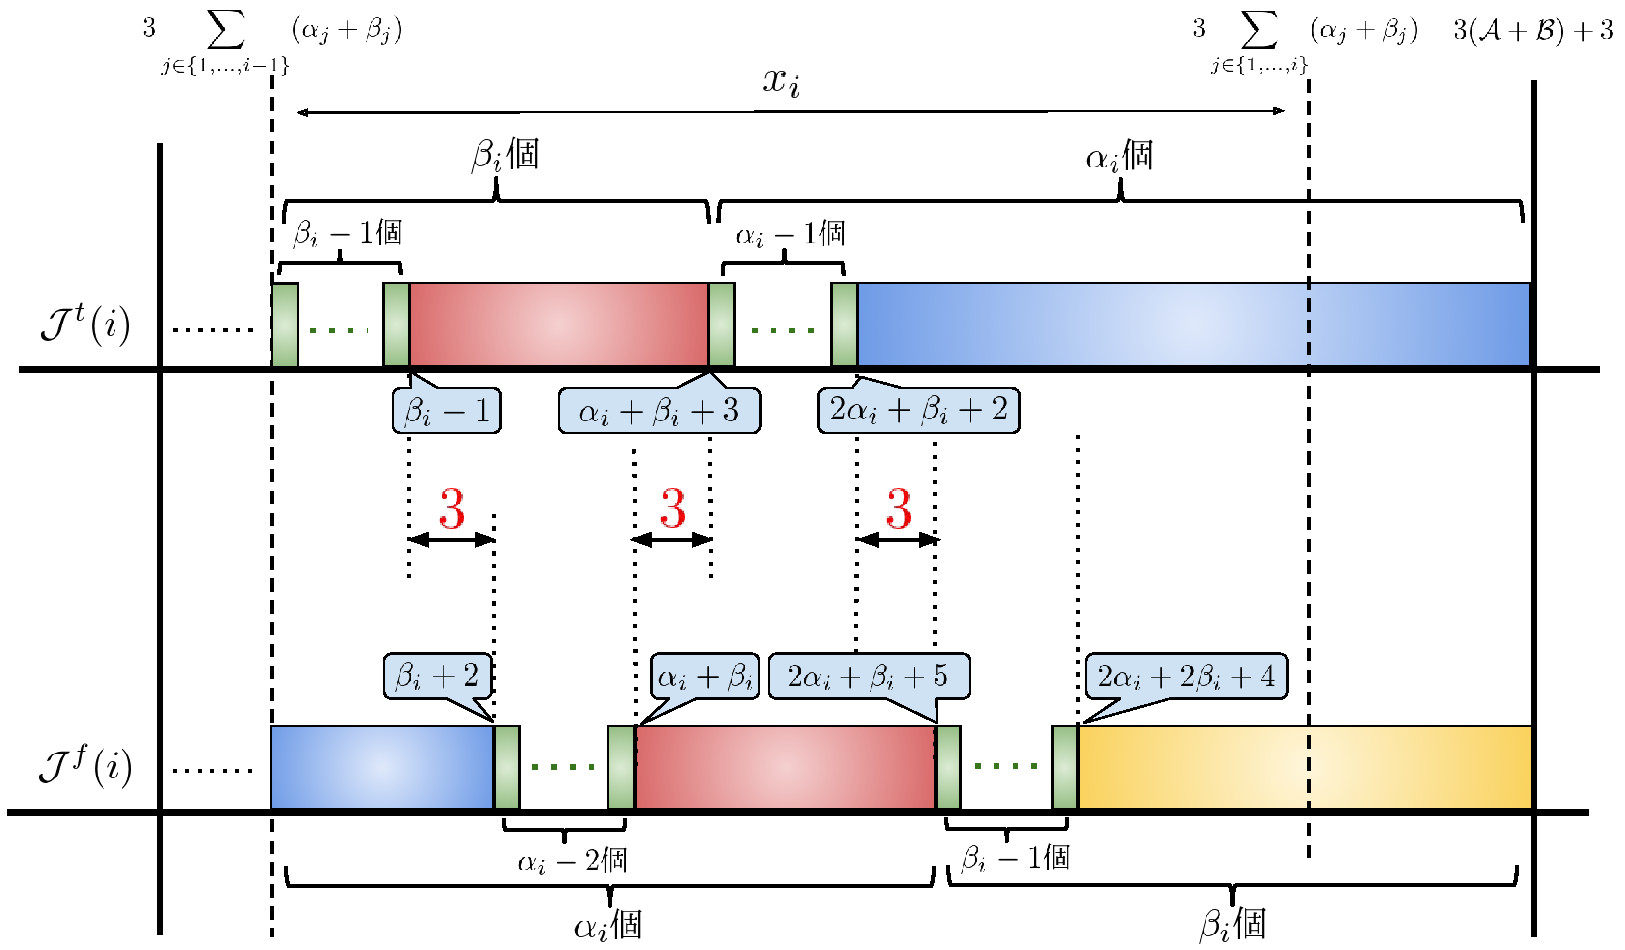
\includegraphics[width = 16cm]{figure/3SAT1.pdf}
  \caption{各 $i \in \{1,\ldots,n\}$ における機械 $i$ に対応するジョブの集合 $\mathcal{J}^t(i)$ または $\mathcal{J}^f(i)$ を機械 $i$ に割り当てたときのスケジュール}
\end{figure}

このように設定した $(\mathcal{J}, \mathcal{M}, r, p, w)$ は待ち時間制約付きスケジューリング問題の入力である.以降,$(X,H)$ に基いて前述のように設定した $(\mathcal{J}, \mathcal{M}, r, p, w)$ を区別して $I_{(X,H)}$ と表す.つまり,$I_{(X,H)} = (\mathcal{J}, \mathcal{M}, r, p, w)$ .

以下, $H$ を充足する真理値割り当て $f : X \to \{0,1\}$ が存在する
ことと,$I_{(X,H)}$ を入力とする待ち時間制約付きスケジューリング問題に対し
て,$\varphi(A,s) \le 2$ を満たす実行可能なスケジュール $(A,s)$ が
存在することが,同値であることを示す.

\begin{lemma}\label{l_6}
  $H$ を充足する真理値割り当て $f : X \to \{0,1\}$ が存在するならば,$I_{(X,H)}$ を入力とする待ち時間制約付きスケジューリング問題に対して $\varphi(A,s) \le 2$ を満たす実行可能なスケジュール $(A,s)$ が存在する.
\end{lemma}

\begin{proof}
  各 $i \in \{1,\ldots, n\}$ について,$f(x_i) = 1$ ならばグループ $n +
  i$ の全てのジョブを,グループ $n + i$ に対応する機械 $i$ に割り当て,
  そうでなければグループ $i$ の全てのジョブを,グループ $i$ に対応する機
  械 $i$ に割り当てる.つまり,各 $i \in \{1,\ldots, n\}$ における各
  $\ell \in \{1,\ldots,\alpha_i + \beta_i\}$ について,
  $f(x_i) = 1$ ならば,$A_i := A_i \cup \mathcal{J}^f(i)$,
  $f(x_i) = 0$ ならば,$A_k := A_k \cup \mathcal{J}^t(i)$ となる.
  $I_{(X,H)}$ の定義より,ここまでのスケジュールにおいて,機械
  $\{1,\ldots, n\}$ に割り当てたジョブは処理開始可能時刻と納期の間で重複せず処理される.
  よって,このとき,機械 $\{1,2,\ldots,n\}$ に割り当てられた
  $\mathcal{A} + \mathcal{B}$ 個のジョブの待ち時間は $0$ である.(図 $4.1$)

  上述の割り当てにより,各 $i \in \{1,\ldots,n\}$ について,$x_i$ または
  $\bar x_i$ に対応するジョブ $\mathcal{J}^t(i)$ または
  $\mathcal{J}^f(i)$ のどちらか一方が機械 $i$ に割り当てられた.このとき,
  上図より,機械 $i$ におけるジョブの完了時刻は $3(\mathcal{A} +
  \mathcal{B}) + 3$ であるので,いずれのジョブも機械 $i$ に割り当てることができない.
  よって,残りのジョブについては,各 $k \in \{n + 1,\ldots,n +
  \lambda\}$ における機械 $k$ に割り当てる.

  前提条件より,$f$ が $H$ を充足することから,各 $i \in \{1,\ldots,n\}$,
  $j \in \{1, \ldots, \lambda \}$ について,$f(x_i) = 1$ を満たす $x_i
  \in h_j$ か,$f(x_i) = 0$ を満たす $\bar x_i \in h_j$ を満たすリテラルは必ず存在する.
  ここで,与えられた $j \in \{1, \ldots, \lambda \}$ について,$f(x_i) =
  1$ を満たす $x_i \in h_j$ を見つけたと仮定する.グループ $i$ のジョブ
  の集合 $\mathcal{J}^t(i)$ は,$f(x_i) = 1$ であることから,
  $\{1,\ldots,n\}$ のいずれの機械にも割り当てられていないので,そのよう
  なグループ $i$ のジョブの集合 $\mathcal{J}^t(i)$ は必ず存在する.
  同様に,$f(x_i) = 0$ を満たす $\bar x_i \in h_j$ を見つけたと仮定する.
  グループ $n + i$ のジョブの集合 $\mathcal{J}^f(i)$ のうち,いずれの機
  械にも割り当てられていないグループ $n + i$ を見つける.先程と同じ議論
  で,そのようなグループ $n + i$ のジョブ $\mathcal{J}^f(i)$ は必ず存在する.

  各 $j \in \{1, \ldots, \lambda \}$ における $h_j$ に対応するジョブの集
  合 $\mathcal{T}(h_j)$ または $\mathcal{F}(h_j)$ のジョブを処理開始可能
  時刻の昇順で機械 $j$ に割り当てる.
  このとき,1 に割り当てられたリテラルに対応するジョブが少なくとも 1 つ
  各機械に割り当てられているので,各機械におけるジョブの完了時刻は高々
  $3(\mathcal{A} + \mathcal{B}) + 2$ である.
  ここで,各 $j \in \{1,\ldots,\lambda\}$ における $J^d(j)$ を各機械 $j$
  に 1 つずつ割り当てる.
  このとき,$J^d$ の処理開始可能時刻は $I_{(X,H)}$ より,$3(\mathcal{A}
  + \mathcal{B})$ であるので,待ち時間は高々 2 である.

  今までの議論より,$\mathcal{A} + \mathcal{B}$ 個のジョブを機械 $i \in
  \{1,\ldots,n\}$ に,$\mathcal{A} + \mathcal{B}$ 個のジョブを機械 $k \in\{n + 1, \ldots, n + \lambda\}$ に,$\lambda$ 個のジョブを機械 $k \in\{n + 1, \ldots, n + \lambda\}$ に割り当てた.
  このとき,全てのジョブをいずれかの機械に割り当てており,全てのジョブに
  関して,待ち時間は高々 2 であることから,$f$ が $H$ を充足す
  るとき,$I_{(X,H)}$ において,$\varphi(A,s) \le 2$ を満たす.
\end{proof}

\begin{lemma}\label{l_7}
  $H$ を充足する真理値割り当て $f : X \to \{0,1\}$ が存在しないならば,$I_{(X,H)}$ を入力とする待ち時間制約付きスケジューリング問題に対して $\varphi(A, C) \le 2$ を満たす実行可能なスケジュール $(A,s)$ が存在しない.
\end{lemma}

\begin{proof}
  $f$ が $H$ を充足しないことから,各 $j \in \{1, \ldots, \lambda \}$ に
  ついて,$f(x_i) = 1$ を満たす $x_i \in h_j$ か,$f(x_i) = 0$ を満たす
  $\bar x_i \in h_j$ が1つも存在しない機械 $j \in \{1,\ldots, \lambda\}$ が必ず存在する.
  その機械を $j^{\prime}$ とし,以下,機械 $j^{\prime}$ 上のスケジュールについて述べる.
  \begin{itemize}
    \item $x_i \in h_{j'}$ または $\bar x_i \in h_{j'}$ に対応
    するジョブのみを機械 $j'$ に割り当てた場合
    $I_{(X,H)}$ の $B.3$ より,それらのジョブは,スケジュールにおける次のジョブの処理開始可能時刻を 1 超える処理時間を持つ.$h_{j'}$ に含
    まれる $x_i$ 以外の残りの 2 つのリテラルに対応するジョブについても
    同様に機械 $j'$ に割り当てる.
    $I_{(X,H)}$ より,機械 $j'$ におけるジョブの完了時刻は
    $3(\mathcal{A} + \mathcal{B}) + 3$ となる.ここで,$j \in
    \{1,\ldots,\lambda\}$ におけるジョブ $J^d(j')$ をそれらの
    ジョブの後に割り当てるとき,ジョブ $J^d(j')$ に 3 の待ち時間が発生する.$|h| = 2,|h| = 1$ のとき,$B.1$ より,それぞれの場合において $J^d \in \mathcal{J}^d$ に 4 または 3 の待ち時間が発生する.(図 4.2)
  \end{itemize}

  \begin{itemize}
    \item $x_k \notin h_j$ または $\bar x_k \notin h_j$ に対応するジョブを
    割り当てた場合

    機械 $j^{\prime}$ にそのようなジョブを1 つでも割り当てた場合,
    $I_{(X,H)}$ より,機械 $j^{\prime}$ におけるジョブの完了時刻は
    $3(\mathcal{A} + \mathcal{B}) + 3$ となる.ここで,$j \in
    \{1,\ldots,\lambda\}$ において,機械に割り当てられていないジョブ
    $J^d(j')$ をそれらのジョブの後に割り当てるとき,ジョブ
    $J^d(j')$ に 3 の待ち時間が発生する.
    \item 上記の 2 つのケースにおいて,$j \in \{1,\ldots,\lambda\}$ におい
    て,機械に割り当てられていないジョブ $J^d(j')$ を機械 $i
    \in \{1,\ldots,n\}$ に割り当てた場合 $I_{(X,H)}$ より,ジョブ
    $J^d(j')$ に 3 の待ち時間が発生する.
  \end{itemize}
  以上より,各 $j \in \{1,\ldots,\lambda\}$ における機械 $j$ にどのジョ
  ブをどのように割り当てたしたとしても,少なくとも 1 つ待ち時間が 3 以上になる機械が存在する.
  よって,$H$ を充足する真理値割り当て $f$ が存在しないとき,待ち時間が 2 以下となるスケジュールは存在しない.
\end{proof}

\begin{figure}[h]
  \centering
  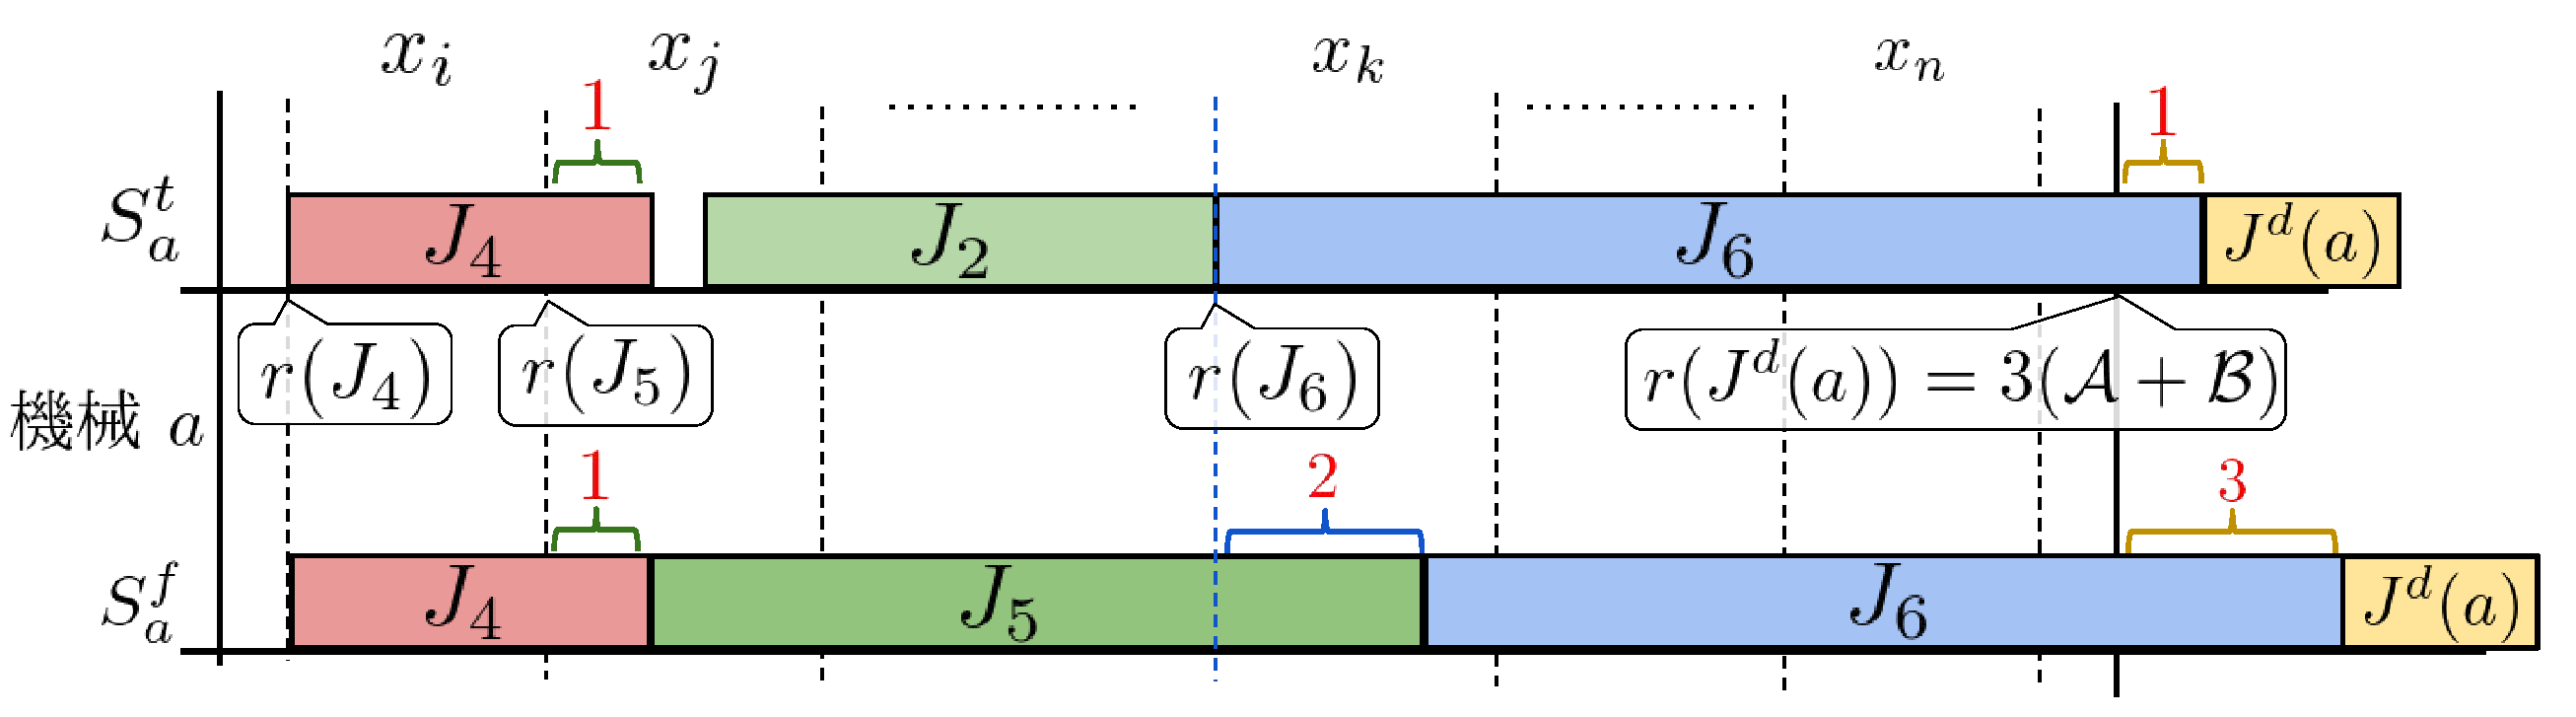
\includegraphics[width = 16cm]{figure/3SAT2.pdf}\\
  \caption{$h_k = (x_i, x_j, x_k)$ のとき,各リテラルに対応するジョブのスケジュール}
\end{figure}

\begin{description}
  \item[スケジュール $S$ ] $x_i = 0, x_j = 1, x_k = 0$ のとき,つまり,$H$ を充足する真理値割り当てが存在する場合.
  \item[スケジュール $S'$ ] $x_i = 0, x_j = 0, x_k = 0$ のとき,つまり,$H$ を充足する真理値割り当てが存在しない場合.
\end{description}

補題~\ref{l_6} と補題~\ref{l_7} より,$H$ を充足する真理値割り当て $f : X \to \{0,
1\}$ が存在することと,$I_{(X,H)}$ を入力とする待ち時間制約付きスケジューリング問題に対して $\varphi(A,s) \le 2$を満たす実行可能なスケジュール $(A,s)$ が存在することは,同値である.3 -SAT 問題の入力 $(X,H)$ に基づく $I_{(X,H)}$ の生成に要する計算時
間は,明らかに多項式時間であり,入力 $I_{(X,H)}$ の長さは,$(X, H)$
の長さに関する多項式で表すことができる.したがって,無関連並列
機械モデルにおいて機械数が入力の一部の場合, 待ち時間制約付きスケジューリング問題は NP 困難である.

ここで,無関連並列機械モデルにおける待ち時間制約付きスケジューリング問題のインスタンスと,スケジュールが与えられたとき,与えられたスケジュールにおける最大待ち時間が $w$ 以下となるかの判定は,明らかに多項式時間で判定可能である.したがって,無関連並列機械モデルにおいて機械数が入力の一部の場合, 待ち時間制約付きスケジューリング問題は NP 困難かつ,NP に属するので,NP 完全である.

また,$H$ を充足する真理値割り当てが存在する場合,待ち時間制約付きスケジューリング問題における最大待ち時間は高々 2 である.
$H$ を充足する真理値割り当てが存在しない場合,待ち時間制約付きスケジューリング問題における最大待ち時間は最小でも 3 である.
したがって,無関連並列機械モデルにおいて機械数が入力の一部の場合,待ち時間制約付きスケジューリング問題が NP 完全である限り,1.5 未満の定数近似アルゴリズムは存在しない.

この証明では,各 $i \in \{1,\ldots,n\}$ において $\alpha_i \ge 3$,$\beta_i \ge 3$ という前提のもと行った.
しかし,各 $i \in \{1,\ldots,n\}$ において $\alpha_i < 3$,$\beta_i < 3$ のときでも,多項式還元可能である.
各 $i \in \{1,\ldots,n\}$ において $\alpha_i$,$\beta_i$ が 3 未満となるリテラルを $x_i$ とすると,$x_i$ を要素とする節と同じ節を $\alpha_i$ もしくは $\beta_i$ が 3 以上となるまで作る.
このとき,新しく作った節は,本来 $H$ の要素である節と同じリテラルを要素とする節であることから,真理値割り当ての結果に影響を与えない,また,真理値割り当ての結果に影響を与えないことから,判定結果にも影響を与えない.
よって,各 $i \in \{1,\ldots,n\}$ において $\alpha_i$,$\beta_i$ が 3 以上となるように,ダミー節を作ることで,この章で紹介した還元方法を適用することができる.

%待ち時間制約付きスケジューリング問題は NP  完全
%最大待ち時間最小化問題は NP 困難である
%なぜなら,・・・・・

\section{最大待ち時間最小化問題の計算複雑さのまとめ}\label{4_s_2}
本研究で,無関連並列機械モデルにおいて,機械数が入力の一部の場合,最大待ち時間最小化問題は,NP 完全であることが明らかになった.しかし,他の機械モデルにおける計算複雑さは明らかになっていない.

しかし,$w = 0$ のとき,この問題は JIT スケジューリング問題に対応し,単一機械モデルと同一機械モデルにおいて,多項式時間で判定できることが明らかになっている.

以下で,単一機械モデルにおける待ち時間制約付きスケジューリング問題について,$w = 0$ のとき,以下の条件を満たすとき,決定問題の解は Yes,満たさないとき No であることは明らかである.
\begin{displaymath}
  \forall J,J' \in \mathcal{J}\bigg[\big[r(J),r(J) + p(J)\big) \cap \big[r(J'),r(J') + p(J')\big) = \emptyset\bigg]
\end{displaymath}

$w = 0$ となるスケジュールとは,すべてのジョブが処理開始可能時刻と 処理開始可能時刻 + 処理時間 の間で処理されなければならない.つまり,すべてのジョブに関して各ジョブの [処理開始可能時刻,処理開始可能時刻 + 処理時間] で表される範囲が被ってはいけない.この判定にかかる時間は高々 $\mathcal{O}(n^2)$ であることから,多項式時間で判定が可能である.
同様に,同一並列機械モデルにおける待ち時間制約付きスケジューリング問題についても多項式で判定可能である.

以下の条件を満たす $\mathcal{J}$ の部分集合 $\mathcal{J}'$ が $|\mathcal{J}'| \le |\mathcal{M}|$ を満たすとき,決定問題の解は Yes,満たさないとき No である.
\begin{displaymath}
  \forall J,J' \in \mathcal{J}'\bigg[\big[s(J),s(J) + p(J)\big) \cap \big[s(J'),s(J') + p(J')\big) \neq \emptyset\bigg]
\end{displaymath}

第 \ref{c_2} 章で紹介した機械モデルの関係より,各機械モデルにおけるスケジューリング問題は,互いに部分問題と拡張問題の関係にある.
つまり,単一機械モデルにおける最大待ち時間最小化問題が NP 完全であれば,残りの機械モデルにおけるスケジューリング問題についても NP 完全であることが言える.
しかし,本研究では,無関連並列機械モデルにおける NP 完全性のみ明らかにしたため,他の機械モデルにおける問題の計算複雑さは明らかでない.

単一機械モデルにおける待ち時間制約付きスケジューリング問題は第~\ref{c_3} 章で紹介した,処理開始可能時刻つき最大遅れ時間最小化問題と対応する.待ち時間制約付きスケジューリング問題において,納期 を処理開始可能時刻と処理時間の和とすると,最大待ち時間は,最大遅れ時間に対応する.したがって,処理開始可能時刻付き最大遅れ時間最小化問題により制限を加えた問題であり,処理開始可能時刻付き最大遅れ時間最小化問題を解くアルゴリズムが存在すれば,最大待ち時間最小化問題も解くことができる.つまり,最大待ち時間最小化問題は処理開始可能時刻付き最大遅れ時間最小化問題の部分問題として捉えることができる.第~\ref{c_3}~章より,処理開始可能時刻付き最大遅れ時間最小化問題が強 NP 困難であることから,最大待ち時間最小化問題も NP 困難であることが予想されるが,本研究では示せていない.そのため,最大待ち時間,最大遅れ時間の 2 つの観点から,単一機械モデルにおける最大待ち時間最小化問題の計算複雑さを明らかにすることは今後の課題である.


\chapter{解法の提案と実験的評価}\label{c_5}
第 \ref{5_s_1} 節では,最大待ち時間最小化問題に対する厳密解法を紹介する.第 \ref{5_s_2} 節では,最大待ち時間最小化問題に対するヒューリスティックを紹介する..第 \ref{5_s_3} 節では,第 \ref{5_s_2} 節で紹介したヒューリスティックの評価と分析を行う.また,第 \ref{5_s_1} 節で紹介した厳密解法の計算時間の分析も行う.

\section{厳密解法の提案}\label{5_s_1}
同一並列機械モデル,無関連並列機械モデルにおける最大待ち時間最小化問題に対する厳密解法を開発した.
第~\ref{c_4}~章で,無関連並列機械モデルにおいて機械数が入力の一部の場合,最大待ち時間最小化問題が NP 完全であることを示した.
NP 困難,完全問題に対する効率的なアルゴリズムは発見されていない.
そのため,NP 困難,完全問題に対する厳密解法の開発においてよく用いられる発想の 1 つに,分枝限定法を用いる,という発想がある.

分枝限定法は最適化問題に対するアルゴリズムを設計するための方法である.この方法は計算時間がどうであろうと,無条件で最適解を見つけたいときに用いる.分枝限定法は,すべての実行可能解の空間をしらみつぶしに探索する手法のバックトラッキングに基づいている.分枝限定法の大まかなアイデアは,しらみつぶし探索において,解を生成するある部分に達したとき,その部分に最適解が含まれていないことがわかったときには,実行可能解の空間のその部分の探索を省略することによってバックトラッキングを早くすることである.

ここで,バックトラッキングを適用するための表記法を導入する.
$\mathcal{M}(x)$ を最適化問題の入力インスタンス $x$ に対するすべての実行可能解の集合とする.$T_{\mathcal{M}(x)}$ を以下のような性質を持つラベル付き木と定義する.
\begin{itemize}
  \item $T_{\mathcal{M}(x)}$ の任意の頂点 $v$ は集合 $S_v \subseteq \mathcal{M}(x)$ によってラベル付けられている.
  \item $T_{\mathcal{M}(x)}$ の根は $\mathcal{M}(x)$ によってラベル付けられている.
  \item $T_{\mathcal{M}(x)}$ において $v_1,\ldots,v_m$ が $v$ の親の全ての子である,つまり,$v$ は $S_v$ の分割である.
  \item $T_{\mathcal{M}(x)}$ の各葉 $u$ に対して,$|S_u| \le 1$.つまり,葉が$\mathcal{M}(x)$ の実行可能解に対応している.
\end{itemize}

バックトラッキングは,ラベルの付いた根付き木 $T_{\mathcal{M}(x)}$ に対する深さ優先探索,あるいは幅優先探索とみなすことができる,ここで葉は $\mathcal{M}(x)$ からの実行可能解でラベル付けされており,$T_{\mathcal{M}(x)}$ の全ての内部頂点 $v$ には,$v$ を根とする部分木 $T_v$ の葉のラベルが付いた全ての実行可能解を含む $S_v \subseteq \mathcal{M}(x)$ でラベル付けされている.分枝限定法は,アルゴリズムが $v$ を訪れた時点で,$T_v$ が最適解を持たないこと決定できるときに,$T_{\mathcal{M}(x)}$ から $T_v$ を切り取ることに他ならない.このアプローチの効率はアルゴリズムの実行中に切断され得る $T_{\mathcal{M}(x)}$ の部分木の量とサイズに依存する.

分枝限定法は多くの NP 困難な組合わせ最適化問題に対して,その最適解を求めるための最も良い
枠組みとして知られており,Land and Doig \cite{BandB} によって
提案され,Little, Murty, Sweeney and Karel \cite{BandB2}
によって TSP にはじめて適用されている.

分枝限定法の最も単純な版は,頂点 $v$ に到達したとき,それまでに見つかった最良のコストと $T_v$
の $S_v$ における実行可能解の最小または最大(ここでは最大)のコストを比較する.それまでの最良のコストが評価された範囲のどのコストよりも明らかに良ければ,$T_v$ を切り取る(すなわち, $T_v$ の探索を中断する).

%図入れたほうがいいかもしれない

この節では,同一並列機械モデルにおける最大待ち時間最小化問題に対する厳密解法に用いた分割生成アルゴリズムと分枝限定法を紹介する.分枝限定法によるアプローチの効率はアルゴリズムの実行中に切断される $T_{\mathcal{M}(x)}$ の部分木の量とサイズ,プログラムに依存する.%また,順列の生成に用いるデータ構造を双方向リストとした.双方向リストの各ノードには 2 つのリンクがあり,1 つが次のノード(ここでは,$.next$ と表記する),もう 1 つが前のノード(ここでは,$.previous$ と表記する)を指す.またここでは,先頭のノードを $head$ と表記し,双方向リストの最後尾のノードの次のノードを $head$,$head$ の前のノードを双方向リストの最後尾のノードとする.

以下では,分割の生成方法,分枝限定法のアルゴリズムと工夫部分について,紹介する.その後,アルゴリズムの紹介を行う.
分割の生成方法については Kreher. Donald L. \cite{rgf} に
よって,紹介されている.

同一並列機械の場合,全ての機械の性能が同じであることから,ジョブをどの機械に割り当てたとしても,処理時間は変わらない.そのため,同一並列機械では,どの機械に割り当てるかではなく,どのジョブと同じ機械で処理するかを考える必要がある.
各ジョブの処理は任意の 1 機械で処理を完了するため,同一並列機械へのジョブの割り当ては,ジョブの分割として捉えることができる.分割の定義は以下の通り.$\mathcal{J}$ の分割 $\Pi$ の要素 $\pi \in \Pi$ に対して,以下の条件を満たす $\Pi$.
\begin{itemize}
  \item $\displaystyle \bigcup_{\pi \in \Pi}\pi = \mathcal{J} $
  \item $\forall \pi, \pi' \in \Pi \big[\pi \neq \pi' \Rightarrow \pi \cap \pi' = \emptyset \big]$
\end{itemize}

%実装部分での工夫と,アルゴリズム部分での工夫は分ける
議論に先立ち,表記を導入する.コストの下限を返す関数を $cost : \mathcal{J} \to \mathbb{N}$ とする.また,$M = \pi$ は分割の要素 $\pi$ に機械 $M$ が対応することを意味する.
\begin{description}
  \item[分割生成アルゴリズムの改良] ~
  \begin{enumerate}
    \setlength{\leftskip}{-10mm}
    \item $|\Pi| = |\mathcal{M}|$ を満たす分割 $\Pi$ のみ生成した.

    機械数が $m$ のとき,生成した分割の要素数が $m$ 未満,または $m$ より多いとき,その分割に対する探索を行う必要がないため,そのような分割を生成しないアルゴリズムに改良することで,考慮する分割を減らすことを可能にした.

    \item 各 $\pi \in \Pi$ における $\mathcal{J}_{\pi}$ のコストの下限 $cost(\mathcal{J}_{\pi})$ を評価し,分割 $\Pi$ において,スケジュールを生成するかどうかの判定を追加した.

    \item 各 $\pi \in \Pi$ における $cost(\mathcal{J}_{\pi})$ を降順でソートし,順に $\pi$ に対応する機械にジョブ $J \in \mathcal{J}_{\pi}$ を割り当てる.

    各 $\pi \in \Pi$ における $cost(\mathcal{J}_{\pi})$ の値が大きい機械から順に割り当てることで,その分割において,目的関数に影響を与える可能性が高いスケジュールから順に考慮することができるため,探索の中断を早い段階で行うことができる.

  \end{enumerate}
  \item[分枝限定法の改良] ~
  \begin{enumerate}
    \setlength{\leftskip}{-10mm}
    \item 部分問題に対する多項式アルゴリズムの概念を導入することで,$cost(\mathcal{J}_{M_a} \setminus \mathcal{J}_{S_{M_a}})$を評価し,探索を続行するか中断するかの判定を追加した.機械 $M_a = \pi \in \Pi$ において,$M_a$ に割り当てられたジョブの集合を $\mathcal{J}_{S_{M_a}}$ とする.

    割り当てられたジョブだけでなく,割り当てられていないジョブに対するコストの下限の評価を加えることで,探索の中断,続行の判定を増やした.
  \end{enumerate}
\end{description}

以下では,上記改良を加えた分割生成アルゴリズムと,分枝限定法の紹介を行う.
議論に先立ち表記の導入を行う.

\begin{itemize}
  \item ジョブの集合 $\mathcal{J} = \{J_1,\ldots,J_n\}$.
  \item 機械の集合 $\mathcal{M} = \{M_1,\ldots,M_m\}$.
  \item ジョブの処理開始可能時刻を返す関数 $r : \mathcal{J} \to \mathbb{N}$.
  \item ジョブの処理時間を返す関数 $p : \mathcal{J} \to \mathbb{N}$.
  \item スケジュールにおける最大待ち時間を返す関数 $w : S \to \mathbb{N}$.
  \item スケジュールにおけるジョブの完了時刻を返す関数 $C : \mathcal{J} \to \mathbb{N}$.
  \item 各 $j \in \{1,\ldots,m\}$ に対する機械 $M_j \in \mathcal{M}$ におけるスケジュール $S_{M_j}$ の集合 $\mathcal{S}$.
  \item それまでのスケジュールにおける最良の解 $W$.
  \item 要素数 $n$ の分割を表す配列 $b$.
  \item 要素数 $n$ の配列 $b_{\max}$ は 各 $1 \le i \le n$ に対して,$i$ 番目の要素は,それまでのジョブが割り当てられた機械の最大数を格納している.つまり,$b_{\max}[i] = \displaystyle \max_{1\le j \le i - 1}b[j]$.
\end{itemize}

\begin{quote}
  \begin{description}
    \item[] ${\mbox {\bf {\sc StrictSolutionMethod}}}$
    \item[入力:] $I = (\mathcal{J},\mathcal{M},r,p,w,C,W)$
    \item[出力:] スケジュールの集合 $\mathcal{S}$
  \end{description}
  \begin{description}
    \item[Step 1.] $(\mathcal{J},\mathcal{M},r,p,C)$ を入力とし,{\sc Heuristic} を実行する.出力を $\mathcal{S}$ とする.このとき,$W = {\displaystyle \max_{S \in \mathcal{S}}w(S)}$ とする.$W = 0$ のとき,スケジュール $\mathcal{S}$ を出力して処理を終了する.
    \item[Step 2.] 組 $(b,b_{\max},n,m)$ を入力として,{\sc increment} を実行し,出力が {\sc false} となるまで,以下の処理を繰り返す.
    \begin{description}
      \item[Step 2.1.] $(b)$ を入力として,{\sc sort} を実行する.
      \item[Step 2.2.] 各 $1 \le i \le n$ に対して,以下の処理を繰り返す.
      \begin{description}
        \item[Step 2.2.1] ジョブの集合 $\mathcal{J}'$ を定義する.ただし $\mathcal{J}' = \emptyset$.
        \item[Step 2.2.2.] 各 $1 \le j \le m$ に対して,以下の処理を繰り返す.
        \begin{description}
          \item[Step 2.2.2.1.] ${\mbox order}[i] = j$ のとき,$\mathcal{J}' :=\mathcal{J}' \cup J_i$ とする.
        \end{description}
        \item[Step 2.2.3.] 組 $(\mathcal{J}',r,p,w,C,0)$ を入力として,{\sc BranchAndBound} を実行する.
        \item[Step 2.2.4.] {\sc BranchAndBound} の出力を $S$ とする.このとき,$\mathcal{S} := \mathcal{S} \cup S$ とする.
      \end{description}
    \end{description}
    \item[Step 3.] スケジュール $\mathcal{S}$ を出力する.
  \end{description}
\end{quote}

上記 \textsc{StrictSolutionMethod} では,\textsc{normalize} と \textsc{increment} により,分割 $\Pi$ の要素数 が 機械数 $m$ と等しくなるように,分割を生成している.その後 \textsc{BranchAndBound} により,各 $\pi \in \Pi$ に対して,順列の生成を行っている.

\begin{quote}
  \begin{description}
    \item[]  ${\mbox {\bf {\sc normalize}}}$
    \item[入力:] $I = (b, b_{\max}, m)$
    \item[出力:] 分割 $b$
  \end{description}
  \begin{description}
    \item[Step 1.] 各 $1 \le i \le n$ に対して,以下の処理を繰り返す.
    \begin{description}
      \item[Step 1.1.] $b_{\max}[n - i] \ge m - i$ のとき,処理を終了する.
      \item[Step 1.2.] $b[n - i] := m - i$,$b_{\max}[n - i] := m - i$
    \end{description}
    \item[Step 2.] $b$ を出力する.
  \end{description}
\end{quote}

上記 {\sc normalize} は,{\sc increment} で生成した $b$ のすべての要素が $m$ 未満のとき,割り当てていない機械が存在するので,その分割 $b$ を $m$ となる要素を少なくとも 1 つ持つ $b$ に変換している.
Step 1.1. では,$n - i$ 番目の 1 つ前のジョブまでが割り当てられた機械番号の最大値が $m$ 以上のとき,すでに要素 $m$ を持っているので,変換せずに出力している.

Step 1.2. 割り当てられていない機械が存在するので,各 $0 \le i \le n - 1$ に対して,$n - i$ から順に $b[n-i] := m - i$ とすることで,分割の要素が $m$ となるように調整している.

\begin{quote}
  \begin{description}
    \item[]  ${\mbox {\bf{\sc increment}}}$
    \item[入力:] $I = (b,b_{\max},n, m)$
    \item[出力:] $b$ が更新されたとき{\sc true} を出力し,それ以外のとき {\sc false} を出力する.
  \end{description}
  \begin{description}
    \item[Step 1.] 各 $n \ge i \ge 1$ に対して以下の処理を繰り返す.
    \begin{description}
      \item[Step 1.1] $b[i] = \min\{b_{\max}[i] + 1, m\}$ のとき,$b[i] := 1$ とする.
      \item[Step 1.2] $b[i] \neq \min\{b_{\max}[i], m\}$ のとき,$b[i] := b[i] + 1$ とする.
      \begin{description}
        \item[Step 1.2.1] $b[i] > b_{\max}[i]$ のとき,各 $i + 1 \le j \le n$ に対して,$b_{\max}[j] := b[i]$ とする.
        \item[Step 1.2.2] $I = (b,b_{\max},m)$ を入力として,{\sc normalize} を実行する.
        \item[Step 1.2.3] {\sc true} を出力する.
      \end{description}
    \end{description}
    \item[Step 2.] {\sc false} を出力する.
  \end{description}
\end{quote}

上記 {\sc increment} は,辞書式順で分割を生成している.配列 $b$ は分割を表しており,$i$ 番目の要素 $b[i]$ は,ジョブ $J_i$ が機械 $b[i]$ に割り当てられていることを表す.ここで,分割の要素数は $\displaystyle \max_{1 \le i \le n}b[i]$ で表すことができる.

Step 1.1. では,各 $n \ge i \ge 1$ における $b[i]$ が $\min\{b_{\max}[i] + 1, m\}$ のとき,それ以上新たな機械を追加することができないので,リセットしてる.

Step 1.2. では,$i$ 番目のジョブを割り当てる機械を新たに追加することができるので,$b[i] := b[i] + 1$ としている.そのとき,Step 1.2.1 で $i$ 番目までの機械の最大数を更新している.

新たな分割を生成したときに,{\sc true} を,生成できなかったときに {\sc false} を返している.

\begin{quote}
  \begin{description}
    \item[] ${\mbox {\bf {\sc sort}}}$
    \item[入力 :] $I = (b)$
    \item[出力 :] 機械への割り当て順を表す配列 ${\mbox order}$
  \end{description}
  \begin{description}
    \item[Step 1.] 要素数 $m$ の配列 ${\mbox cost}$ と ${\mbox order}$ を定義する.ただし,$1 \le j \le m $ に対して,${\mbox order}[j] = j$ とする.
    \item[Step 2.] 各 $1 \le i \le n$ に対して,以下の処理を繰り返す.
    \begin{description}
      \item[Step 2.1.] ジョブの集合 $\mathcal{J}'$ を定義する.ただし $\mathcal{J}' = \emptyset$.
      \item[Step 2.2.] $1 \le j \le m$ に対して以下の処理を繰り返す.
      \begin{description}
        \item[Step 2.2.1.] $b[i] = j$ のとき,$\mathcal{J}' :=\mathcal{J}' \cup J_i$ とする.
      \end{description}
      \item[Step 2.3.] $I = (\mathcal{J}',S_{M_j})$ を入力として,{\sc evaluation} を実行する.
      \item[Step 2.4.] {\sc evaluation} により出力されたスケジュールを $S'_{M_j}$ とし,\\${\mbox cost}[j] := w(S'_{M_j})$ とする.
    \end{description}
    \item[Step 3.] ${\mbox cost}$ の降順となるように,${\mbox order}$ をソートする.
    \item[Step 4.] ${\mbox order}$ を出力する.
  \end{description}
\end{quote}

\begin{quote}
  \begin{description}
    \item[] ${\mbox {\bf {\sc evaluation}}}$
    \item[入力 :] $I = (\mathcal{J'},S)$
    \item[出力 :] スケジュール $S$
  \end{description}
  \begin{description}
    \item[Step 1.] 各 $1 \le i \le |\mathcal{J}'|$ における $J'_i$ に対して,以下の処理を繰り返す.
    \begin{description}
      \item[Step 1.1.] $p(J'_i) = \displaystyle \min_{j \in \{1,\ldots,|\mathcal{J}'|\}}p(J'_j)$ とする.
      \item[Step 1.2.] $S := S \cup J'_i$ とする.
    \end{description}
    \item[Step 2.] $S$ を出力する.
  \end{description}
\end{quote}

上記 {\sc evaluation} は,機械に割り当てられていないジョブの集合 $\mathcal{J}'$ について,部分問題に対する多項式アルゴリズムを用いて,解を求めている.

それまでのスケジュールにおける最良の解のコスト $W$ と,スケジュールされていない残りのジョブを最適にスケジュールして得られた解 $w'$ を比較して $W \le w'$ であれば,探索を中断することができ,効率を上げることができる.ここで,最適なスケジュールの求める方法として,第 \ref{c_3} 章で紹介した部分問題に対する多項式アルゴリズムを用いる.
また,残りのジョブを本来の処理時間で最適にスケジュールして得られる解を $W_{opt}$ とする.

すべてのジョブに関して,処理時間が一定のとき,処理開始可能時刻の昇順で処理することで最適なスケジュールが求まる.このとき,{\sc evaluation} では全てのジョブの処理時間を残りのジョブの最小の処理時間 $p_{\min}$ とした.
ここで,残りのすべてのジョブの中で最大の処理時間を $p_{\max}$ としたとき,すべてのジョブの処理時間 $p$は $p_{\min} \le p \le p_{\max}$ である.ここで,,設定する処理時間が $p_{\min}$ より大きいとき,設定した処理時間より小さい値を持つジョブが少なくとも 1 つ存在する.このとき,$w' < W_{opt}$ とならない可能性がある.$W_{opt} < w'$ のとき,最低でも $w'$ 以上のコストがかかることを表しているので,最適なスケジュールを含む部分木を切り取ってしまう可能性がある.そのため,残りのジョブの処理時間を $p_{\min}$ として設定することで,最適なスケジュールを含む部分木を切り取ることなく探索できる.

\begin{quote}
  \begin{description}
    \item[] ${\mbox {\bf {\sc BranchAndBound}}}$
    \item[入力 :] $I = (\mathcal{J}',r,p,w,C,W,i)$
    \item[出力 :] スケジュール $S$
  \end{description}
  \begin{description}
    \item[] $i = |\mathcal{J}'|$ のとき,
    \begin{description}
      \item[Step 1.] $W = w(S)$ とし,スケジュール $S$ を出力する.
    \end{description}
    \item[] $i \neq |\mathcal{J}'|$ のとき,
    \begin{description}
      \item[Step 2.] $\mathcal{J}'$ を処理開始可能時刻の昇順でソートする.
      \item[Step 3.] 各 $1 \le j \le |\mathcal{J}'|$ における $J'_j$ に対して,以下の処理を繰り返す.
      \begin{description}
        \item[Step 3.1] $S := S \cup J'_j$ とし,$\mathcal{J}'$ から $J'_j$ を取り除く.
        \item[Step 3.2] $\mathcal{J}'$ に対して,$(\mathcal{J}',S)$ を入力
        として,{\sc evaluation} を適用し,出力されたスケジュールを $S'$ とする.
        \begin{description}
          \item[Step 3.2.1] $W \le w(S')$ のとき,$(\mathcal{J}',r,p,w,C,W,i + 1)$ を入力として {\sc BranchAndBound} を実行する.
        \end{description}
        \item[Step 3.3] $J'_j$ を $\mathcal{J}'$ の取り除いた場所に
        戻す.
      \end{description}
    \end{description}
  \end{description}
\end{quote}

% BranchAndBound の説明
上記 {\sc BranchAndBound} は,再帰的に順列の生成を行っている.
Step 3.2. では,機械に割り当てられていないジョブの集合 $\mathcal{J}'$ に対して,部分問題に対する多項式アルゴリズムを用いて出力したスケジュール $S'$ における最大待ち時間 $w(S')$ がそれまでの最良の解 $W$ より良いとき,探索を続行している.
全てのジョブをスケジュールしたとき,Step 1. で解の更新を行っている.それ以降の探索は更新した解を用いて判定を行う.

\section{ヒューリスティックの提案}\label{5_s_2}
本研究では,同一並列機械モデル,無関連並列機械モデルにおける最大待ち時間最小化問題に対して,貪欲アルゴリズムを用いた解法を提案する.
貪欲アルゴリズムとは,最適化問題に対する最も単純なアルゴリズムの 1 つとして知られており,Juraj Hromkovic [2004] \cite{greedy} で紹介されている.
バックトラッキングや局所探索と類似点は,実行可能解($p_1\ldots,p_n$)($i \in \{1,\ldots,n\}[p_i \in P_i]$)の仕様が必要であり,任意の貪欲アルゴリズムは局所ステップの系列と見ることができる点である.しかし,貪欲アルゴリズムは 1 つの実行可能解からもう 1 つの実行可能解には遷移しない.まず,空の状態から始まり,仕様における 1 つの局所パラメータを永久に確定する.第 2 ステップでは,局所アルゴリズムは仕様における第 2 のパラメータを確定する.この操作が実行可能解の完全な仕様に到達するまで繰り返される.貪欲アルゴリズムは,次の局所仕様を生成するために全ての可能性の中から最も有望と思われるパラメータを選択する.後で,どのような状況が起ころうと,この決定は決して変えられることはない.
また,貪欲アルゴリズムはバックトラッキングで生成される木$T_{\mathcal{M}(x)}$ における根から葉までのちょうど 1 つの路を実現している.空仕様は全ての実行可能解の集合 $\mathcal{M}(x)$ を考えており,$\mathcal{M}(x)$ が木 $T_{\mathcal{M}(x)}$ における根のラベルであるこ
とを意味している.第 1 のパラメータ $p_1$ を指定することは,$\mathcal{M}$ を集合 $S(p_1) = \{\alpha \in \mathcal{M}(x) \mid \alpha \text{ の仕様の第 1 パラメータは } p_1\}$ に制限することに対応する.この手続きを繰り返すと,実行可能解の集合の系列

\begin{displaymath}
  S(p_1,p_2,\ldots,p_n) \subseteq \ldots, \subseteq S(p_1,p_2) \subseteq S(p_1) \subseteq \mathcal{M}(x)
\end{displaymath}

を得る.ここで,$|S(p_1,p_2,\ldots,p_n)| = 1$ である.\\

\noindent 以下の {\sc Heuristic} は,同一並列機械モデルにおける最大待ち時間最小化問題に対する提案解法である.議論に先立ち表記を導入する.

\begin{itemize}
  \item ジョブの集合 $\mathcal{J} = \{J_1,\ldots,J_n\}$.
  \item 機械の集合 $\mathcal{M} = \{M_1,\ldots,M_m\}$.
  \item ジョブの処理開始可能時刻を返す関数 $r : \mathcal{J} \to \mathbb{N}$.
  \item ジョブの処理時間を返す関数 $p : \mathcal{J} \to \mathbb{N}$.

  ただし,無関連並列機械モデルのとき,$p : \mathcal{J} \times \mathcal{M} \to \mathbb{N}$ となる.
  \item スケジュールにおける最大待ち時間を返す関数 $w : S \to \mathbb{N}$.
  \item スケジュールにおける完了時刻を返す関数 $C : S \to \mathbb{N}$.
  \item スケジュール $S$ はジョブの順列を表す.
  \item 各 $M \in \mathcal{M}$ におけるスケジュール $S_M$ の集合 $\mathcal{S}$.
  つまり,$\mathcal{S} = \{S_M \mid M \in \mathcal{M}\}$.
\end{itemize}

\begin{quote}
  \begin{description}
    \item[] ${\mbox {\bf {\sc Heuristic}}}$
    \item[入力 :] $I = (\mathcal{J}, \mathcal{M},r,p,C)$
    \item[出力 :] スケジュールの集合 $\mathcal{S}$.
  \end{description}
  \begin{description}
    \item[Step 1.]
    $\mathcal{J}$ を処理開始可能時刻の昇順でソートする.
    \item[Step 2.]
    各機械 $M \in \mathcal{M}$ におけるスケジュールを $S_M \in \mathcal{S}$ と表記する.
    ただし,$\forall M, M' \in \mathcal{M}\big[M \neq M' \Rightarrow S_M \cap S_{M'} = \emptyset \big]$,$\displaystyle \bigcup_{S \in \mathcal{S}}S = \mathcal{S}$を満たす.つまり,$S_M$ は $\mathcal{S}$ の分割である.
    \item[Step 3.]
    各 $1 \le i \le n$ における $J_i$ について以下の処理を繰り返す.
    \begin{description}
      \item[Step 3.1.]
      最小完了時刻を持つスケジュール集合の要素 $S_{M_a} \in {\displaystyle \left\{\argmin_{M \in \mathcal{M}}C(S_M)\right\}}$ を 1 つ求める.
      ここで,$S_{M_a} := S_{M_a} \cup J_i$ とする.
    \end{description}
    \item[Step 4.]
    $\mathcal{S} = \{ S_M \mid M \in \mathcal{M}\}$ として,$\mathcal{S}$ を出力する.
  \end{description}
\end{quote}

上記 {\sc Heuristic} は,処理開始可能時刻が最も早いジョブから順に,処理をしていない機械,または処理が一番早く終わった機械に割り当てる.

Step 1.で,処理開始可能時刻が最も早いジョブから順に,処理をしていない機械,または処理が一番早く終わった機械に割り当てる.
Step 3. で,処理をしていない機械,または処理が一番早く終わった機械 におけるスケジュールを取得し $S_{M_a}$ と定義している.その後,スケジュール $S_{M_a}$ にジョブ $J_i$ を追加する.

本研究での提案解法は貪欲アルゴリズムに基づいた解法である.
あるインスタンスに対する最適解から得られる最大待ち時間が 0 だった場合,本研究での提案解法により出力される最大待ち時間も 0 になる.Cepek and Sung \cite{JIT} を参考に,その証明を紹介する.

\begin{lemma}
  あるインスタンスに対する最適解から得られた最大待ち時間が $0$ のとき,貪欲アルゴリズムに基づいた本研究での提案解法により出力された解から得られた最大待ち時間も $0$ になる.
\end{lemma}

\begin{proof}
  待ち時間制約付きスケジューリング問題において,$w = 0$ のとき,すべてのジョブは JIT ジョブである.このとき JIT ジョブ荷重和最大化問題においても,$W = {\displaystyle \sum_{J \in \mathcal{J}}w(J)}$ となるスケジュールが存在する.
  ここで,JIT ジョブ荷重和最大化問題におけるすべてのジョブが JIT ジョブのとき,貪欲アルゴリズムに基づいた解法により,最適解,つまり,$W = {\displaystyle \sum_{J \in \mathcal{J}}w(J)}$ となるスケジュールを作ることができると Cepek and Sung [2004] \cite{JIT} により証明されている.
  したがって,最大待ち時間最小化問題においても,すべてのジョブが JIT ジョブのとき,貪欲アルゴリズムに基づいた解法で,最適解を求めることができる.
\end{proof}

\section{提案解法の評価と分析}\label{5_s_3}
同一並列機械モデル,無関連並列機械モデルにおける最大待ち時間最小化問題に対して,本研究で提案したヒューリスティックの実験的評価を行った.評価方法は,各インスタンスに対して,本研究で提案するアルゴリズムにより出力された解から得られた最大待ち時間 $W_h$ と,厳密解法により出力された最適解から得られた最大待ち時間 $W_{opt}$ を比較するものである.ここで,$\max\{W_h/W_{opt}\}$ を競合比という.

実験結果の紹介に先立ち,競合比の値の取りうる幅について紹介する.
\begin{table}[htb]
  \begin{center}
    \begin{tabular}{|c|c|c|c|c|c|c|} \hline
      $\mathcal{J}$ & $J_1$ & $J_2$ & $J_3$ & $J_4$ & $J_5$ & $J_6$\\
      \hline \hline
      $r(J)$ & 2 & 3 & 11 & 16 & 23 & 26 \\ \hline
      $p(J)$ & 8 & 7 & 11 & 10 & 10 & 11\\ \hline
    \end{tabular}
    \caption{各ジョブにおける処理開始可能時刻と処理時間}
  \end{center}
\end{table}

表 5.1 と同一並列機械の集合 $\mathcal{M} (|\mathcal{M}| = 2)$ がインスタンスとして与えられたとき,最適なスケジュールとそうでないスケジュールは以下の通り.
\begin{description}
  \item[最適なスケジュール $\mathcal{S}$] $S_1 : (J_1, J_3, J_5)$,$S_2 : (J_2, J_4, J_6)$.このとき,$w(\mathcal{S}) = 0$ となる.ただし,$\mathcal{S} = S_1 \cup S_2$.
  \item[最適でないスケジュール $\mathcal{S}'$] $S'_1 : (J_1, J_3, J_6)$,$S'_2 : (J_2, J_4, J_5)$.このとき,$w(\mathcal{S}') = 3$ となる.ただし,$\mathcal{S}' = S'_1 \cup S'_2$.
\end{description}

上記のとき,$\text{競合比} = \infty$ となる.つまり,最適でないスケジュールを生成したアルゴリズムの質は無限大となる.
また,$w(\mathcal{S}) = w(\mathcal{S}')$ のとき,競合比 = 1 となる.つまり,本研究の実験において競合比は 1 から $\infty$ の値のいずれかを取る.
しかし,第 \ref{5_s_2} 節の証明より,本研究で提案したヒューリスティックでは,最適解から得られた最大待ち時間が 0 のとき,ヒューリスティックから出力された解から得られる最大待ち時間も 0 になる.したがって,本研究で提案したアルゴリズムの質は定数で収まることが保証されている.以上に基づいた実験結果は以下の通り.
\begin{description}
  \item[厳密解法の評価] ~
  \begin{description}
    \item[尺度 1 :] インスタンスサイズの増加に伴う,分割生成アルゴリズムの改良前と改良後の計算時間の比較
    %
    \item[尺度 2 :] インスタンスサイズの増加に伴う,分枝限定法の改良前と改良後の計算時間の比較
    %
    \item[ヒューリスティックの評価] ~
    \begin{description}
      \item[尺度 3 :] 各インスタンスにおけるジョブの処理時間幅の増加に伴う競合比の変動
      %
      \item[尺度 4 :] 各インスタンスにおけるジョブの処理時間幅の増加に伴う計算時間の変動
      %
      \item[尺度 5 :] インスタンスサイズの増加に伴う,同一並列機械モデルと無関連並列機械モデルの競合比の比較
      %
      \item[尺度 6 :] インスタンスサイズの増加に伴う,同一並列機械モデルと無関連並列機械モデルの計算時間の比較
      %
    \end{description}

  \end{description}
\end{description}

\chapter{結論}\label{c_6}
\section{研究成果}
本研究では,最大待ち時間最小化問題に関して以下の成果を得た.
\begin{description}
  \item[成果 1:]
  最大待ち時間最小化問題を決定問題として定義したとき,無関連並列機械モデルにおいて機械数が入力の一部の場合,最大待ち時間最小化問題 の NP 完全性を明らかにした.

  JIT ジョブ荷重和最大化問題における \textsc{3-SAT} からの還元手法に着目し,最大待ち時間最小化問題 の NP 完全性を示した.

  \item[成果 2:]
  同一並列機械モデル,無関連並列機械モデルにおける最大待ち時間最小化問題に対する厳密解法を開発し,解法に対する計算時間の評価を行った.

  NP 困難な問題に対する効率的な解法は発見されていない.
  そのため,最適解を求めるためには,実行可能解を全列挙し比較する必要がある.
  そこで,本研究では,最大待ち時間最小化問題に対する厳密解法に分割生成アルゴリズムと分枝限定法を用いた.

  同一並列機械モデルでは,ジョブの機械への割り当てに対応する分割生成アルゴリズムに対し,分割の要素数 = 機械数 となる改良を加えた.
  無関連並列機械モデルでは,上記の改良を加えた分割に対して,ジョブに対応する機械の入れ替えを加えることで,ジョブの機械への割り当てを実現させた.この改良により,考慮する分割の数を減らし,計算効率を向上させた.

  また,分枝限定法に処理開始可能時刻付き最大遅れ時間最小化問題の部分問題に対する多項式アルゴリズムの概念を導入した.この改良により,列挙する順列を減らし,計算効率を向上させた.
  その結果,同じインスタンスに対して,計算時間を約 ??? 倍にすることに成功した.

  \item[成果 3:]
  同一並列機械モデル,無関連並列機械モデルにおける最大待ち時間最小化問題に対するヒューリスティックを開発し,実験的評価を行った.

  貪欲的解法に基づいたヒューリスティックを開発した.
  ヒューリスティックによる解から得られた目的関数の値を $W_h$,厳密解法による最適解より得られた目的関数の値を $W_{opt}$ とすると,異なるインスタンスに対して,$W_h/W_{opt}$ を求めることで,提案解法の評価を行った.$W_h/W_{opt}$ の値が 1 に近いほど,解法の質は良いと言える.本研究の実験によると,$\max\big\{W_h/W_{opt}\big\} = ?$ の結果を得た.

  \item[まとめ:] 本研究では,無関連並列機械モデルにおいて,機械数が入力の一部の場合,最大待ち時間最小化問題が NP 完全であることを証明した.しかし,単一機械モデル,同一並列機械モデル,一様並列機械モデルにおける計算複雑さは明らかでない.本研究で示した還元方法が,その他の機械モデルにおける計算複雑さの証明の足がかりになるものと期待する.
\end{description}

\section{今後の課題}
\begin{description}
  \item[計算複雑さ:] 本研究で,無関連並列機械モデルにおいて,機械数が入力の一部の場合,最大待ち時間最小化問題は NP 完全であることを証明した.
  しかし,単一機械モデル,同一並列機械モデル,一様並列機械モデルにおける計算複雑さは明らかでない.これらの機械モデルにおける計算複雑さを明らかにし,問題の難しさに与える影響の特徴づけは,今後の課題である.

  \item[還元方法の工夫:] 本研究で開発した解法は,解の質を保証しないヒューリスティックである.
  計算複雑さの証明より,無関連並列機械モデルにおいて,機械数が入力の一部の場合,1.5 未満の定数近似ができないことを示した.還元方法を工夫し,{\sc 3-SAT} の存在判定が Yes の場合と No の場合の最大待ち時間の比率を調整することができれば,より定数近似ができないと言える幅を広げることができる.これは,今後の課題である.

  \item[解法:]
  還元方法の工夫の成果に基づき,近似アルゴリズムを開発することも今後の課題である.
  {\sc 3-SAT} の存在判定が Yes の場合と No の場合の最大待ち時間の比率が大きいほど,最大待ち時間最小化問題の難しさをより強めることができる.また,その比率に応じた近似アルゴリズム,もしくは,多項式時間近似スキームの開発も今後の課題である.

\end{description}
\addcontentsline{toc}{chapter}{\bibname}
\bibliographystyle{splncs03}
\bibliography{thesis}

\appendix
\chapter{付録}\label{c_7}
約 320 万回の実験で,同一並列機械モデル,無関連並列機械モデルにおける最大待ち時間最小化問題 に対し,
\begin{displaymath}
  \max \left\{ \frac{\text{ヒューリスティックによる解から得られた最大待ち時間}}{\text{最適解から得られた最大待ち時間}}\right\}
\end{displaymath}

と,厳密解法の計算時間を,各ジョブ数,各機械数,処理時間の上限をもとに行なった結果である.\ref{5_s_3}~節の解法の評価では,以下の表を参照している.

\begin{table}[htb]
  \begin{center}
    \begin{tabular}{|c|c|c|c|} \hline
      ジョブ数 & 機械数 & 改良前 & 改良後 \\ \hline \hline
      & 2 & 53 & 3  \\ \cline{2-4}
      10 & 3 & 109 & 24  \\ \cline{2-4}
      & 4 & 249 & 101  \\ \cline{2-4}
      & 5 & 553 & 146  \\ \hline \hline
      & 2 & 470 & 7  \\ \cline{2-4}
      11 & 3 & 857 & 76 \\ \cline{2-4}
      & 4 & 1,798 & 475  \\ \cline{2-4}
      & 5 & 3,436 & 943  \\ \hline \hline
      & 2 & 4,543 & 25  \\ \cline{2-4}
      12 & 3 & 8,086 & 250  \\ \cline{2-4}
      & 4 & 15,523 & 2,085 \\ \cline{2-4}
      & 5 & 30,271 & 7,576   \\ \hline \hline
      & 2 & 62,609 & 145 \\ \cline{2-4}
      13 & 3 & 107,357 & 872 \\ \cline{2-4}
      & 4 & 158,662 & 8,865 \\ \cline{2-4}
      & 5 & 240,917 & 40,748 \\ \hline \hline
      & 2 & 767,835 & 677 \\ \cline{2-4}
      14 & 3 & 1,246,264 & 3,889 \\ \cline{2-4}
      & 4 & 2,091,361 & 39,538 \\ \cline{2-4}
      & 5 & 3,121,089 & 249,759  \\ \hline \hline
    \end{tabular}
    \caption{分割生成アルゴリズムの改良前と改良後の厳密解法の計算時間(単位:ms)}
  \end{center}
\end{table}

\begin{table}[htb]
  \begin{center}
    \begin{tabular}{|c|c|c|c|} \hline
      ジョブ数 & 機械数 & 改良前 & 改良後 \\ \hline \hline
      & 2 & 8 & 3  \\ \cline{2-4}
      10 & 3 & 32 & 23  \\ \cline{2-4}
      & 4 & 131 & 99  \\ \cline{2-4}
      & 5 & 313 & 168  \\ \hline \hline
      & 2 & 33 & 6  \\ \cline{2-4}
      11 & 3 & 120 & 74 \\ \cline{2-4}
      & 4 & 597 & 477  \\ \cline{2-4}
      & 5 & 1,709 & 971  \\ \hline \hline
      & 2 & 188 & 25  \\ \cline{2-4}
      12 & 3 & 470 & 243  \\ \cline{2-4}
      & 4 & 2,672 & 2,044 \\ \cline{2-4}
      & 5 & 9,758 & 6,887   \\ \hline \hline
      & 2 & 1,101 & 110 \\ \cline{2-4}
      13 & 3 & 2,041 & 834 \\ \cline{2-4}
      & 4 & 12,194 & 8,887 \\ \cline{2-4}
      & 5 & 54,966 & 43,903 \\ \hline \hline
      & 2 & 7,118 & 649 \\ \cline{2-4}
      14 & 3 & 9,534 & 2,890 \\ \cline{2-4}
      & 4 & 56,564 & 37,492 \\ \cline{2-4}
      & 5 & 295,287 & 225,043  \\ \hline \hline
      & 2 & 48,458 & 3,361 \\ \cline{2-4}
      15 & 3 & 49,636 & 1,012 \\ \cline{2-4}
      & 4 & 269,089 & 160,610 \\ \cline{2-4}
      & 5 & 1,668,411 & 1,301,890  \\ \hline \hline
    \end{tabular}
    \caption{分枝限定法の改良前と改良後の厳密解法の計算時間(単位:ms)}
  \end{center}
\end{table}

\begin{table}[htb]
  \begin{center}
    \begin{tabular}{|c|c|c|c|c|c|c|c|c|} \hline
       &  & \multicolumn{5}{c|}{処理時間の上限} \\ \hline
      ジョブ数 & 機械数& 10 & 20 & 30 & 40 & 50 \\ \hline \hline
       & 2 & 8 & 12 & 11 & 5.5 & 6.7   \\ \cline{2-7}
       10 & 3 & 3 & 11 & 11 & 22 & 12.5   \\ \cline{2-7}
       & 4 & 3 & 3.7 & 7 & 10 &  9  \\ \cline{2-7}
       & 5 & 2 & 1.5 & 2.7 & 6 & 13   \\ \hline \hline

       & 2 & 7 & 11 & 15 & 6.5 & 7   \\ \cline{2-7}
       11 & 3 & 5 & 10 & 13 & 24 & 14 \\ \cline{2-7}
       & 4 & 3 & 6 & 11 & 9 & 7.5   \\ \cline{2-7}
       & 5 & 1 & 2 & 6 & 7 & 8   \\ \hline \hline

       & 2 & 8 & 13 & 7 & 9 & 4.5   \\ \cline{2-7}
       12 & 3 & 5 & 10 & 8.5 & 15 & 14.5 \\ \cline{2-7}
       & 4 & 2 & 5 & 10 & 14 & 15   \\ \cline{2-7}
       & 5 & 2 & 3 & 5 & 12 & 14  \\ \hline \hline

       & 2 & 8 & 10 & 14 & 3.9 & 4.3 \\ \cline{2-7}
       13 & 6 & 8 & 10 & 14 & 9.7 & 15 \\ \cline{2-7}
       & 4 & 2 & 7 & 7 & 13 & 6 \\ \cline{2-7}
       & 5 & 1.5 & 5 & 5 & 9 & 9 \\ \hline \hline

       & 2 & 8 & 7 & 7.5 & 3 & 3.2 \\ \cline{2-7}
       14 & 3 & 5 & 9 & 10 & 9.5 & 6 \\ \cline{2-7}
       & 4 &  &  &  &  &  \\ \cline{2-7}
       & 5 &  &  &  &  &  \\ \hline \hline

       & 2 & 8 & 9 & 3.7 & 3.4 & 3.7 \\ \cline{2-7}
       15 & 3 & 6 & 10 & 13 & 10 & 6 \\ \cline{2-7}
       & 4 &  &  &  &  &  \\ \cline{2-7}
       & 5 &  &  &  &  &  \\ \hline \hline

       & 2 & 8 & 7 & 4 & 2.8 & 2.2 \\ \cline{2-7}
       16 & 3 & 5 & 13 & 9 & 7.4 & 3.2 \\ \cline{2-7}
       & 4 &  &  &  &  &  \\ \cline{2-7}
       & 5 &  &  &  &  &  \\ \hline \hline

       & 2 & 8 & 7 & 4 & 2.8 & 2.6 \\ \cline{2-7}
       17 & 3 &  &  &  &  &  \\ \cline{2-7}
       & 4 &  &  &  &  &  \\ \cline{2-7}
       & 5 &  &  &  &  &  \\ \hline \hline
      \end{tabular}
    \caption{同一並列機械モデルにおけるヒューリスティックの競合比}
  \end{center}
\end{table}

% \begin{table}[htb]
%   \begin{center}
%     \begin{tabular}{|c|c|c|c|c|c|c|c|c|c|} \hline
%       機械数/ジョブ数 & 処理時間の上限 & 10 & 11 & 12 & 13 & 14 & 15 & 16 & 17 \\ \hline \hline
%       & 10 & 8 & 7 & 8 & 8 & 8 & 8 & 8 & 8 \\ \cline{2-10}
%       & 20 & 12 & 11 & 13 & 10 & 7 & 9 & 7 & 7 \\ \cline{2-10}
%       2 & 30 & 11 & 15 & 7 & 14 & 7.5 & 3.7 & 4 & 4 \\ \cline{2-10}
%       & 40 & 5.5 & 6.5 & 9 & 3.9 & 3 & 3.4 & 2.8 & 2.8 \\ \cline{2-10}
%       & 50 & 6.7 & 7 & 4.5 & 4.3 & 3.2 & 3.7 & 2.2 & 2.6 \\ \hline \hline
%       & 10 & 3 & 5 & 5 & 6 & 5 & 6 & 5 &  \\ \cline{2-10}
%       & 20 & 11 & 10 & 10 & 8 & 9 & 10 & 13 &  \\ \cline{2-10}
%       3 & 30 & 11 & 13 & 8.5 & 10 & 10 & 13 & 9 &  \\ \cline{2-10}
%       & 40 & 22 & 24 & 15 & 9.7 & 9.5 & 10 & 7.4 &  \\ \cline{2-10}
%       & 50 & 12.5 & 14 & 14.5 & 15 & 6 & 6 & 3.2 &  \\ \hline \hline
%       & 10 & 3 & 3 & 2 & 2 &  &  &  & \\ \cline{2-10}
%       & 20 & 3.7 & 6 & 5 & 7 &  &  &  &  \\ \cline{2-10}
%       4 & 30 & 7 & 11 & 10 & 7 &  &  &  &  \\ \cline{2-10}
%       & 40 & 10 & 9 & 14 & 13 &  &  &  &  \\ \cline{2-10}
%       & 50 & 9 & 7.5 & 15 & 6 &  &  &  &  \\ \hline \hline
%       & 10 & 2 & 1 & 2 & 1.5 &  &  &  &  \\ \cline{2-10}
%       & 20 & 1.5 & 2 & 3 & 5 &  &  &  &  \\ \cline{2-10}
%       5 & 30 & 2.7 & 6 & 5 & 5 &  &  &  &  \\ \cline{2-10}
%       & 40 & 6 & 7 & 12 & 9 &  &  &  &  \\ \cline{2-10}
%       & 50 & 13 & 8 & 14 & 9 &  &  &  &  \\ \hline \hline
%     \end{tabular}
%     \caption{同一並列機械モデルにおけるヒューリスティックの競合比}
%   \end{center}
% \end{table}

\begin{table}[htb]
  \begin{center}
    \begin{tabular}{|c|c|c|c|c|c|c|c|c|} \hline
       &  & \multicolumn{5}{c|}{処理時間の上限} \\ \hline
      ジョブ数 & 機械数& 10 & 20 & 30 & 40 & 50 \\ \hline \hline
       & 2 & 0.3 & 0.5 & 0.6 & 0.8 & 0.9   \\ \cline{2-7}
       10 & 3 & 0.4 & 2.4 & 5.2 & 8.6 & 14   \\ \cline{2-7}
       & 4 & 0.3 & 3.3 & 11 & 24 & 37   \\ \cline{2-7}
       & 5 & 0.05 & 0.8 & 4.8 & 13 & 29   \\ \hline \hline

       & 2 & 1.2 & 2.3 & 2.9 & 3.5 & 4.5   \\ \cline{2-7}
       11 & 3 & 3.6 & 19 & 36 & 47  & 54 \\ \cline{2-7}
       & 4 & 2.3 & 23 & 73 & 135 & 199   \\ \cline{2-7}
       & 5 & 0.5 & 9.5 & 46 & 127 & 239   \\ \hline \hline

       & 2 & 3.1 & 5.6 & 7 & 9.6 & 15   \\ \cline{2-7}
       12 & 3 & 17 & 78 & 134 & 166 & 185 \\ \cline{2-7}
       & 4 & 12 & 139 & 429 & 749 & 1.024   \\ \cline{2-7}
       & 5 & 3.6 & 76 & 385 & 1,008 & 1,886  \\ \hline \hline

       & 2 & 7.8 & 13 & 18 & 31 & 60 \\ \cline{2-7}
       13 & 3 & 73 & 311 & 491 & 590 & 654 \\ \cline{2-7}
       & 4 & 91 & 876 & 2,448 & 3,968 & 4,940 \\ \cline{2-7}
       & 5 & 31 & 710 & 3,168 & 7,751 & 12,093 \\ \hline \hline

       & 2 & 17 & 29 & 47 & 108 & 275 \\ \cline{2-7}
       14 & 3 & 269 & 1,049 & 1,535 & 1,728 & 1,796 \\ \cline{2-7}
       & 4 &  &  &  &  &  \\ \cline{2-7}
       & 5 &  &  &  &  &  \\ \hline \hline

       & 2 & 33 & 76 & 163 & 548 & 1,696 \\ \cline{2-7}
       15 & 3 & 1,151 & 4,116 & 5,811 & 6,744 & 7,649 \\ \cline{2-7}
       & 4 &  &  &  &  &  \\ \cline{2-7}
       & 5 &  &  &  &  &  \\ \hline \hline

       & 2 & 89 & 188 & 595 & 3,099 & 11,308 \\ \cline{2-7}
       16 & 3 & 4,737 & 14,861 & 19,667 & 21,928 & 24,588 \\ \cline{2-7}
       & 4 &  &  &  &  &  \\ \cline{2-7}
       & 5 &  &  &  &  &  \\ \hline \hline

       & 2 & 251 & 545 & 3,148 & 20,600 & 83,626 \\ \cline{2-7}
       17 & 3 &  &  &  &  &  \\ \cline{2-7}
       & 4 &  &  &  &  &  \\ \cline{2-7}
       & 5 &  &  &  &  &  \\ \hline \hline
      \end{tabular}
    \caption{同一並列機械モデルにおける厳密解法の計算時間}
  \end{center}
\end{table}

%
% \begin{table}[htb]
%   \setlength{\leftskip}{-15mm}
%   \begin{tabular}{|c|c|c|c|c|c|c|c|c|c|} \hline
%     機械数/ジョブ数 & 処理時間の上限 & 10 & 11 & 12 & 13 & 14 & 15 & 16 & 17 \\ \hline \hline
%     & 10 & 0.3 & 1.2 & 3.1 & 7.8 & 17 & 33 & 89 & 251 \\ \cline{2-10}
%     & 20 & 0.5 & 2.3 & 5.6 & 13 & 29 & 76 & 188 & 545 \\ \cline{2-10}
%     2 & 30 & 0.6 & 2.9 & 7 & 18 & 47 & 163 & 595 & 3,148 \\ \cline{2-10}
%     & 40 & 0.8 & 3.5 & 9.6 & 31 & 108 & 548 & 3,099 & 20,600 \\ \cline{2-10}
%     & 50 & 0.9 & 4.5 & 15 & 60 & 275 & 1,696 & 11,308 & 83,626 \\ \hline \hline
%     & 10 & 0.4 & 3.6 & 17 & 73 & 269 & 1,151 & 4,737 &  \\ \cline{2-10}
%     & 20 & 2.4 & 19 & 78 & 311 & 1,049 & 4,116 & 14,861 &  \\ \cline{2-10}
%     3 & 30 & 5.2 & 36 & 134 & 491 & 1,535 & 5,811 & 19,667 &  \\ \cline{2-10}
%     & 40 & 8.6 & 47 & 166 & 590 & 1,728 & 6,744 & 21,928 &  \\ \cline{2-10}
%     & 50 & 14 & 54 & 185 & 654 & 1,796 & 7,649 & 24,588 &  \\ \hline \hline
%     & 10 & 0.3 & 2.3 & 12 & 91 &  &  &  & \\ \cline{2-10}
%     & 20 & 3.3 & 23 & 139 & 876 &  &  &  &  \\ \cline{2-10}
%     4 & 30 & 11 & 73 & 429 & 2,448 &  &  &  &  \\ \cline{2-10}
%     & 40 & 24 & 135 & 749 & 3,968 &  &  &  &  \\ \cline{2-10}
%     & 50 & 37 & 199 & 1,024 & 4,940 &  &  &  &  \\ \hline \hline
%     & 10 & 0.05 & 0.5 & 3.6 & 31 &  &  &  &  \\ \cline{2-10}
%     & 20 & 0.8 & 9.5 & 76 & 710 &  &  &  &  \\ \cline{2-10}
%     5 & 30 & 4.8 & 46 & 385 & 3,168 &  &  &  &  \\ \cline{2-10}
%     & 40 & 13 & 127 & 1,008 & 7,751 &  &  &  &  \\ \cline{2-10}
%     & 50 & 29 & 239 & 1,886 & 12,093 &  &  &  &  \\ \hline \hline
%   \end{tabular}
%   \caption{同一並列機械モデルにおける厳密解法の計算時間(単位:ms)}
% \end{table}

\begin{table}[htb]
  \begin{center}
    \begin{tabular}{|c|c|c|c|c|c|c|c|c|} \hline
       &  & \multicolumn{5}{c|}{処理時間の上限} \\ \hline
      ジョブ数 & 機械数& 10 & 20 & 30 & 40 & 50 \\ \hline \hline
       & 2 &  &  &  &  &    \\ \cline{2-7}
       10 & 3 &  &  &  &  &    \\ \cline{2-7}
       & 4 &  &  &  &  &    \\ \cline{2-7}
       & 5 &  &  &  &  &    \\ \hline \hline
       & 2 &  &  &  &  &    \\ \cline{2-7}
       11 & 3 &  &  &  &   &  \\ \cline{2-7}
       & 4 &  &  &  &  &    \\ \cline{2-7}
       & 5 &  &  &  &  &    \\ \hline \hline
       & 2 &  &  &  &  &    \\ \cline{2-7}
       12 & 3 &  &  &  &  &  \\ \cline{2-7}
       & 4 &  &  &  &  &    \\ \cline{2-7}
       & 5 &  &  &  &  &   \\ \hline \hline
       & 2 &  &  &  &  &  \\ \cline{2-7}
       13 & 3 &  &  &  &  &  \\ \cline{2-7}
       & 4 &  &  &  &  &  \\ \cline{2-7}
       & 5 &  &  &  &  &  \\ \hline \hline
       & 2 &  &  &  &  &  \\ \cline{2-7}
       14 & 3 &  &  &  &  &  \\ \cline{2-7}
       & 4 &  &  &  &  &  \\ \cline{2-7}
       & 5 &  &  &  &  &  \\ \hline \hline
       & 2 &  &  &  &  &  \\ \cline{2-7}
       15 & 3 &  &  &  &  &  \\ \cline{2-7}
       & 4 &  &  &  &  &  \\ \cline{2-7}
       & 5 &  &  &  &  &  \\ \hline \hline
       & 2 &  &  &  &  &  \\ \cline{2-7}
       16 & 3 &  &  &  &  &  \\ \cline{2-7}
       & 4 &  &  &  &  &  \\ \cline{2-7}
       & 5 &  &  &  &  &  \\ \hline \hline
       & 2 &  &  &  &  &  \\ \cline{2-7}
       17 & 3 &  &  &  &  &  \\ \cline{2-7}
       & 4 &  &  &  &  &  \\ \cline{2-7}
       & 5 &  &  &  &  &  \\ \hline \hline
      \end{tabular}
    \caption{無関連並列機械モデルにおけるヒューリスティックの競合比}
  \end{center}
\end{table}

\begin{table}[htb]
  \begin{center}
    \begin{tabular}{|c|c|c|c|c|c|c|c|c|} \hline
       &  & \multicolumn{5}{c|}{処理時間の上限} \\ \hline
      ジョブ数 & 機械数& 10 & 20 & 30 & 40 & 50 \\ \hline \hline
       & 2 &  &  &  &  &    \\ \cline{2-7}
       10 & 3 &  &  &  &  &    \\ \cline{2-7}
       & 4 &  &  &  &  &    \\ \cline{2-7}
       & 5 &  &  &  &  &    \\ \hline \hline
       & 2 &  &  &  &  &    \\ \cline{2-7}
       11 & 3 &  &  &  &   &  \\ \cline{2-7}
       & 4 &  &  &  &  &    \\ \cline{2-7}
       & 5 &  &  &  &  &    \\ \hline \hline
       & 2 &  &  &  &  &    \\ \cline{2-7}
       12 & 3 &  &  &  &  &  \\ \cline{2-7}
       & 4 &  &  &  &  &    \\ \cline{2-7}
       & 5 &  &  &  &  &   \\ \hline \hline
       & 2 &  &  &  &  &  \\ \cline{2-7}
       13 & 3 &  &  &  &  &  \\ \cline{2-7}
       & 4 &  &  &  &  &  \\ \cline{2-7}
       & 5 &  &  &  &  &  \\ \hline \hline
       & 2 &  &  &  &  &  \\ \cline{2-7}
       14 & 3 &  &  &  &  &  \\ \cline{2-7}
       & 4 &  &  &  &  &  \\ \cline{2-7}
       & 5 &  &  &  &  &  \\ \hline \hline
       & 2 &  &  &  &  &  \\ \cline{2-7}
       15 & 3 &  &  &  &  &  \\ \cline{2-7}
       & 4 &  &  &  &  &  \\ \cline{2-7}
       & 5 &  &  &  &  &  \\ \hline \hline
       & 2 &  &  &  &  &  \\ \cline{2-7}
       16 & 3 &  &  &  &  &  \\ \cline{2-7}
       & 4 &  &  &  &  &  \\ \cline{2-7}
       & 5 &  &  &  &  &  \\ \hline \hline
       & 2 &  &  &  &  &  \\ \cline{2-7}
       17 & 3 &  &  &  &  &  \\ \cline{2-7}
       & 4 &  &  &  &  &  \\ \cline{2-7}
       & 5 &  &  &  &  &  \\ \hline \hline
      \end{tabular}
    \caption{無関連並列機械モデルにおける厳密解法の計算時間(単位:ms)}
  \end{center}
\end{table}

\chapter*{謝辞}
本研究を進めるにあたり指導教員の宋教授には,研究に対する助言や熱心な指導をしていただきましたことを心から感謝致します.またゼミや日常で多くの知識や示唆をいただいた高橋先生,吉山先輩,田中先輩,丹羽先輩,牧石先輩と研究室の同期の方々に深く感謝致します

\begin{flushright}
  2018年1月31日 \氏名
\end{flushright}
\endmatter
\end{document}
